\documentclass[conference]{IEEEtran}
\IEEEoverridecommandlockouts

% ===================== Packages =====================
\usepackage{cite}
\usepackage{amsmath,amssymb,amsfonts}
\usepackage{algorithmic}
\usepackage{graphicx}
\usepackage{textcomp}
\usepackage{xcolor}
\usepackage{booktabs}
\usepackage{array}
\usepackage[caption=false,font=footnotesize]{subfig}
\usepackage{placeins}

% Tighter float spacing for two-column report
\setlength{\textfloatsep}{6pt plus 1pt minus 2pt}
\setlength{\floatsep}{5pt plus 1pt minus 2pt}
\setlength{\intextsep}{6pt plus 1pt minus 2pt}
\renewcommand{\topfraction}{0.95}
\renewcommand{\dbltopfraction}{0.95}
\renewcommand{\floatpagefraction}{0.85}
\renewcommand{\dblfloatpagefraction}{0.85}

% ===================== Title / Authors =====================
\title{COMP0222 Coursework 02: Visual and LiDAR SLAM}

\author{
\IEEEauthorblockN{Group Code: TODO}
\IEEEauthorblockA{
Department of Computer Science\\
University College London\\
London, United Kingdom}
}

\begin{document}
\maketitle
\raggedbottom

% ===================== Abstract =====================
\begin{abstract}
This report presents our experiments for COMP0222 Coursework 02. We evaluate visual SLAM on public datasets and on self-collected monocular sequences, and we evaluate 2D LiDAR SLAM on self-collected laser scans. For the self-collected visual SLAM task, we acquire one indoor and one outdoor RGB sequence, reconstruct them with COLMAP, track them with monocular ORB-SLAM2, and compare the estimated camera trajectories using EVO. For the LiDAR task, we analyse laser odometry, mapping, loop closure detection, and factor graph optimisation.
\end{abstract}

\begin{IEEEkeywords}
Visual SLAM, LiDAR SLAM, ORB-SLAM2, COLMAP, EVO, monocular camera, trajectory evaluation
\end{IEEEkeywords}

% ============================================================
\section{Visual SLAM with Public Datasets}
\label{sec:q1_public_datasets}

% TODO: Insert Question 1 content here.
% Suggested structure:
% \subsection{Dataset Description}
% \subsection{Baseline Evaluation}
% \subsection{Effect of ORB Feature Number}
% \subsection{Effect of Outlier Rejection}
% \subsection{Effect of Loop Closure}
% \subsection{Discussion}

This section is reserved for Question 1. It should include the KITTI 07 and TUM monocular ORB-SLAM2 experiments, the EVO evaluation plots, the tested parameter settings, and a discussion of how ORB feature number, outlier rejection, and loop closure affect trajectory quality.

% ============================================================
\section{Visual SLAM with Our Own Sequences}
\label{sec:q2_visual_slam}

\subsection{Overview}

For Question 2, we collected two monocular RGB video streams: one indoor sequence and one outdoor sequence. Both were captured as continuous image streams rather than disconnected still images. We used COLMAP for camera calibration refinement, sparse reconstruction, and camera trajectory extraction. The same sequences were then tracked using monocular ORB-SLAM2 with fixed RealSense D455 calibration. Finally, EVO was used to compare the ORB-SLAM2 trajectories against the refined COLMAP trajectories.

Since no external motion-capture, LiDAR, or survey-grade ground truth was available for these self-collected sequences, the EVO results should be interpreted as agreement with COLMAP rather than absolute metric accuracy. Sim(3) alignment was used because both COLMAP and ORB-SLAM2 are monocular pipelines and therefore have arbitrary global scale.

\subsection{Data Collection and Calibration}

\subsubsection{Acquisition Strategy}

The data were collected using the colour stream of an Intel RealSense D455 camera at $848 \times 480$ resolution and 30 FPS. During capture, the camera was hand-carried at approximately constant height and moved slowly through each environment. We deliberately used translational motion rather than pure yaw rotation, because monocular reconstruction requires parallax for reliable triangulation. Sudden turns were avoided where possible to reduce motion blur and preserve feature overlap between consecutive frames.

The indoor sequence, \textit{indoor\_02}, was captured in a large office/atrium area containing tables, chairs, white walls, glass doors, carpet, repeated planar structures, and occasional people. The outdoor sequence, \textit{outdoor\_01}, was captured in a covered courtyard/walkway with tables, poles, barriers, signs, glass facades, and building edges. Representative frames are shown in Fig.~\ref{fig:q2_raw_frames}.

\begin{figure}[!t]
\centering
\subfloat[Indoor.]{
    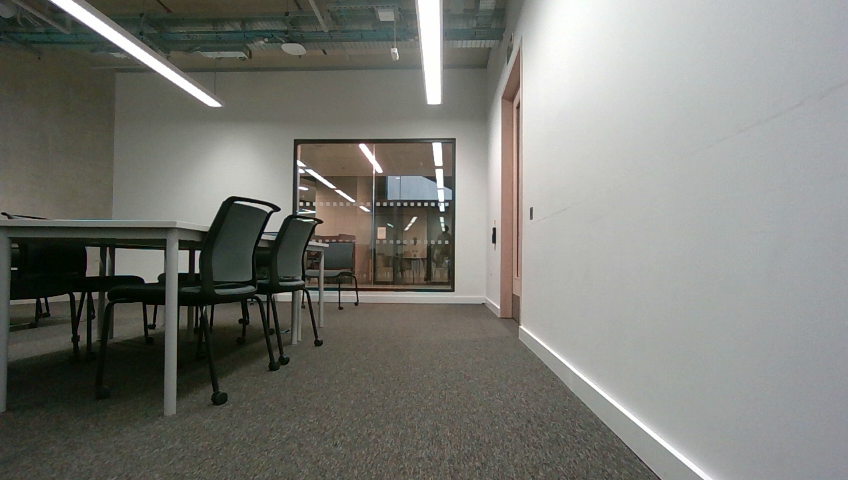
\includegraphics[width=0.48\linewidth]{images/Q2/figures/raw_frames/indoor_000000.png}
}
\hfill
\subfloat[Indoor.]{
    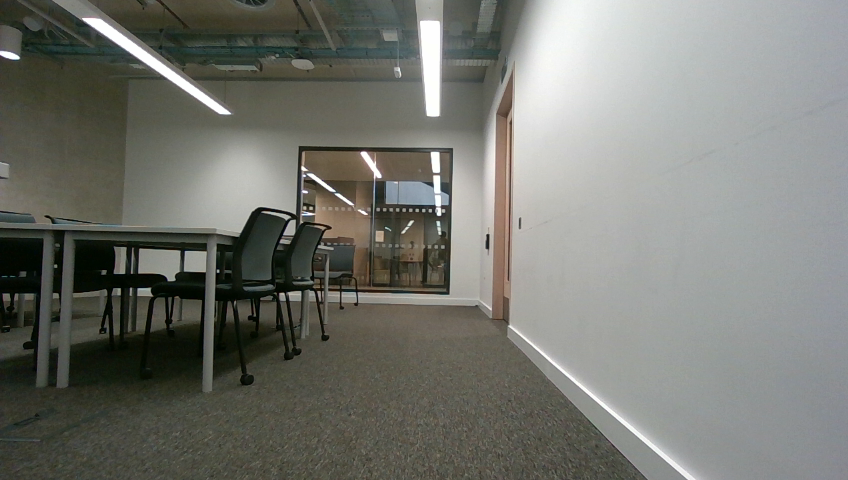
\includegraphics[width=0.48\linewidth]{images/Q2/figures/raw_frames/indoor_001242.png}
}

\vspace{1mm}

\subfloat[Outdoor.]{
    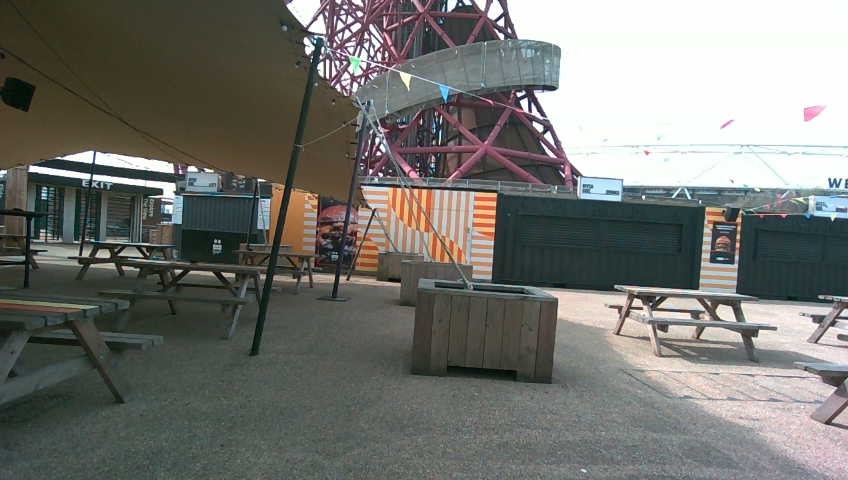
\includegraphics[width=0.48\linewidth]{images/Q2/figures/raw_frames/outdoor_000000.png}
}
\hfill
\subfloat[Outdoor.]{
    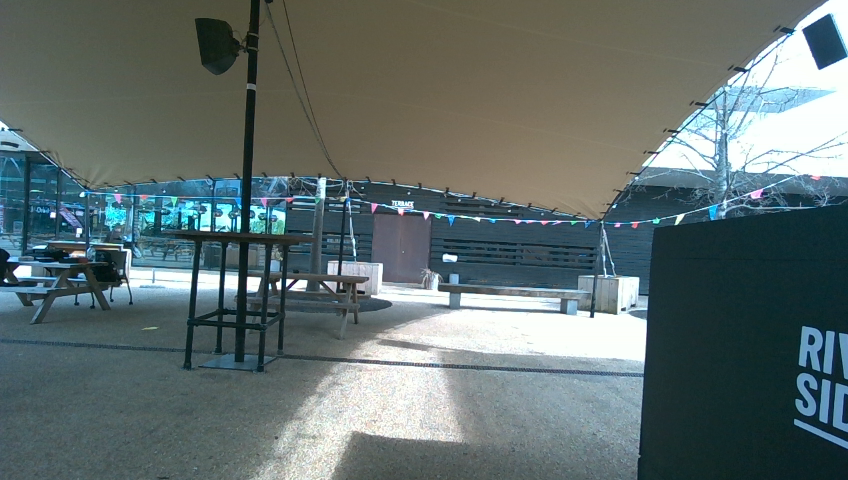
\includegraphics[width=0.48\linewidth]{images/Q2/figures/raw_frames/outdoor_002119.png}
}
\caption{Representative frames from the self-collected monocular streams. The indoor sequence contains larger low-texture planar regions, while the outdoor sequence provides stronger geometric edges and more stable visual structure.}
\label{fig:q2_raw_frames}
\end{figure}

Table~\ref{tab:q2_sequence_stats} summarises the capture and image-quality statistics. Both sequences contain more than 500 frames after ORB-SLAM2 initialisation. The outdoor sequence has much higher Laplacian blur variance and more good inter-frame matches, indicating sharper images and more stable feature correspondences.

\begin{table}[!t]
\caption{Capture and processing statistics for the self-collected monocular sequences. Blur is measured using Laplacian variance; brightness is mean grey value.}
\centering
\footnotesize
\begin{tabular}{lcc}
\toprule
Quantity & Indoor & Outdoor \\
\midrule
Resolution & \multicolumn{2}{c}{$848 \times 480$} \\
Frame rate & \multicolumn{2}{c}{30 FPS} \\
Raw frames & 2222 & 3275 \\
Duration (s) & 74.1 & 109.1 \\
COLMAP sampled images & 600 & 600 \\
COLMAP registered images & 600 & 600 \\
ORB-SLAM2 input frames & 2218 & 3269 \\
Frames after initialisation & $>$500 & $>$500 \\
Mean blur & 301.8 & 1049.5 \\
Mean brightness & 116.8 & 109.9 \\
Mean ORB features & 1099.0 & 1200.0 \\
Mean good matches & 259.9 & 425.9 \\
\bottomrule
\end{tabular}
\label{tab:q2_sequence_stats}
\end{table}

\subsubsection{Calibration and Processing Settings}

The RealSense SDK factory intrinsics were read at the capture resolution and used as the fixed ORB-SLAM2 calibration. COLMAP used a shared FULL OPENCV camera model initialised from the D455 intrinsics and refined it during bundle adjustment. The refined focal lengths remained close to the factory values: indoor $f_x = 429.677$, $f_y = 429.681$; outdoor $f_x = 428.907$, $f_y = 428.471$. The final bundle-adjustment costs were 0.517 px for indoor and 0.425 px for outdoor, supporting the validity of the initial calibration.

ORB-SLAM2 was run in monocular mode on the full filtered streams. Loop closing and outlier rejection were kept enabled. The configuration used 2000 ORB features, scale factor 1.2, 8 pyramid levels, and FAST thresholds 20/7. The camera parameters used in the ORB-SLAM2 YAML file are shown in Table~\ref{tab:q2_orbslam_yaml}.

\begin{table}[!t]
\caption{ORB-SLAM2 monocular configuration used for both self-collected sequences.}
\centering
\footnotesize
\begin{tabular}{lc}
\toprule
YAML parameter & Value \\
\midrule
Camera.fx & 426.7957 \\
Camera.fy & 426.2545 \\
Camera.cx & 427.2596 \\
Camera.cy & 250.0979 \\
Camera.k1 & -0.05605 \\
Camera.k2 & 0.06574 \\
Camera.p1 & -0.000917 \\
Camera.p2 & 0.000815 \\
Camera.k3 & -0.02142 \\
Camera.fps & 30 \\
ORBextractor.nFeatures & 2000 \\
ORBextractor.scaleFactor & 1.2 \\
ORBextractor.nLevels & 8 \\
FAST thresholds & 20 / 7 \\
\bottomrule
\end{tabular}
\label{tab:q2_orbslam_yaml}
\end{table}

COLMAP was run on sampled image streams to keep reconstruction tractable while preserving route coverage. We used every 3rd frame for the indoor stream and every 5th frame for the longer outdoor stream, capped at 600 images per sequence. Sequential matching was used because the data were captured as ordered video streams. The sparse COLMAP model was used for trajectory extraction because COLMAP estimates camera poses during sparse structure-from-motion and bundle adjustment. Dense reconstruction was not used for trajectory evaluation.

\subsection{Indoor Sequence}

The indoor sequence was successfully reconstructed and tracked, but it was the more challenging case. COLMAP registered all 600 sampled images and recovered the overall loop-like route. However, the scene contains white walls, glass, carpet, repeated planar structures, and occasional moving people. These factors reduce distinctive long-term feature tracks and can create ambiguous feature matches.

Fig.~\ref{fig:q2_indoor_summary} summarises the indoor result. The COLMAP sparse model is valid for trajectory extraction because all sampled images were registered and the global route structure was recovered. ORB-SLAM2 also produced a coherent sparse map and exported 158 keyframes with 10,859 sparse map points. The EVO comparison shows that the ORB-SLAM2 trajectory follows the same route as COLMAP, but with larger local deviations around weak-texture and repeated-structure regions. The indoor APE RMSE is 0.1221 and the RPE RMSE is 0.0281.

\begin{figure*}[!t]
\centering
\subfloat[COLMAP sparse top view.]{
    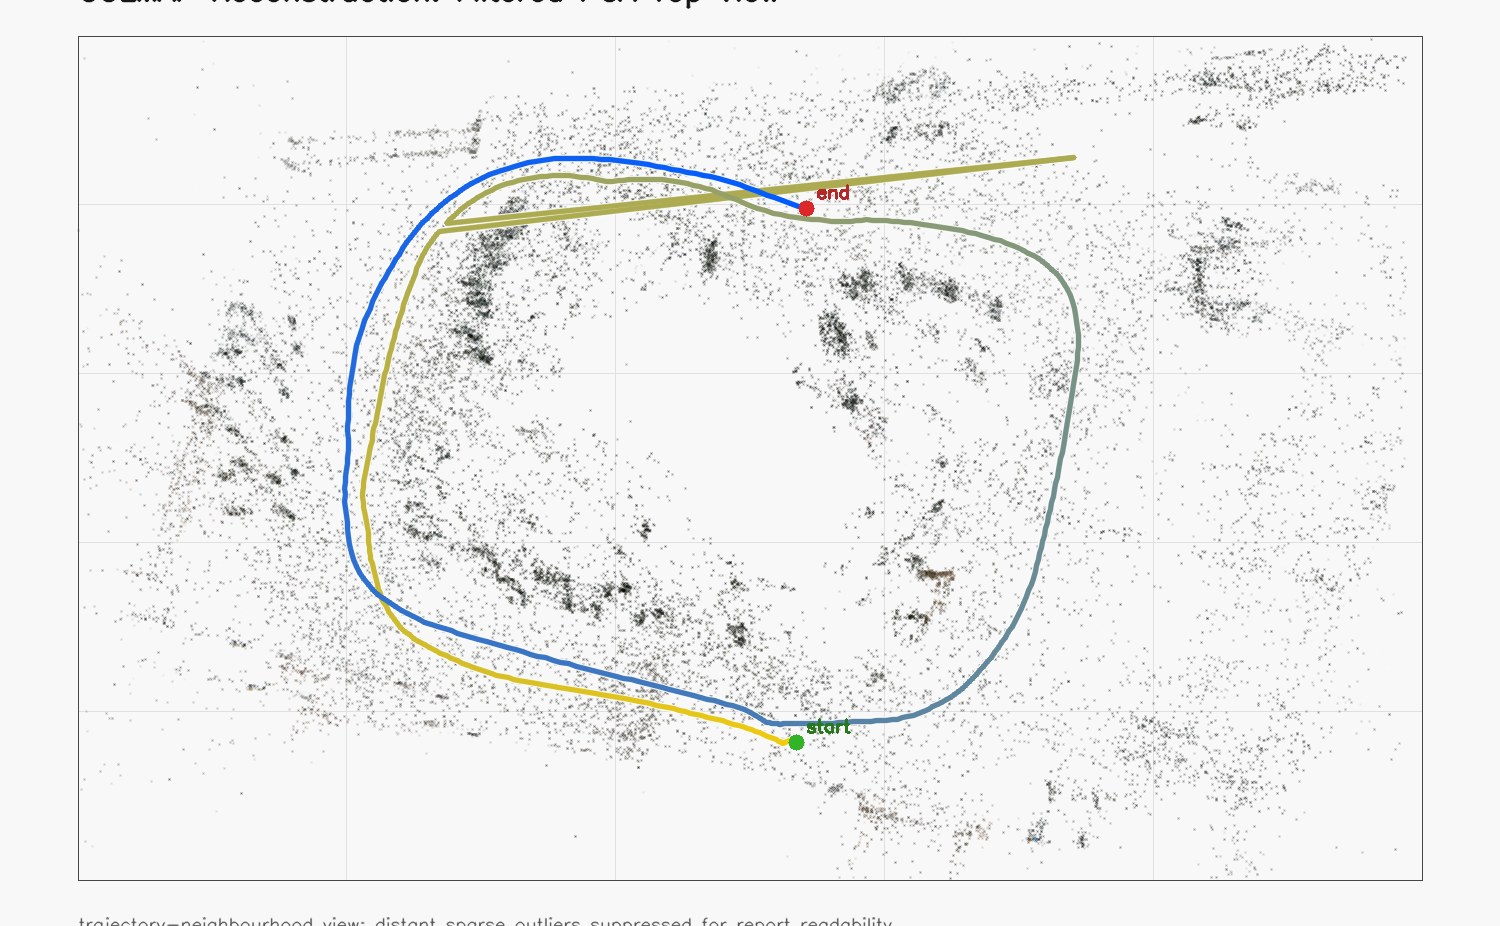
\includegraphics[width=0.24\textwidth]{images/Q2/figures/colmap/indoor_02/sparse_top_view.png}
}
\hfill
\subfloat[ORB-SLAM2 sparse top view.]{
    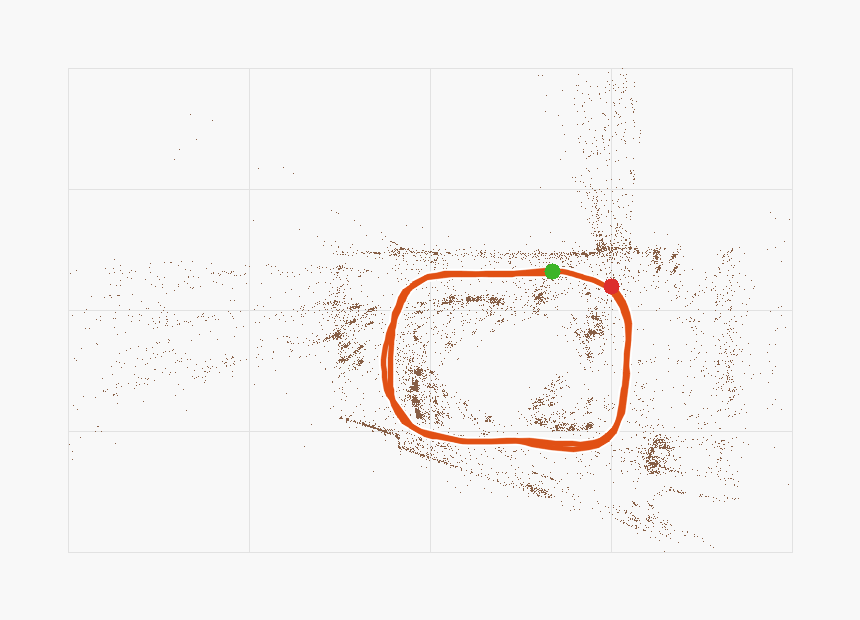
\includegraphics[width=0.24\textwidth]{images/Q2/figures/orbslam/indoor_02/indoor_map_top_view.png}
}
\hfill
\subfloat[EVO trajectory overlay.]{
    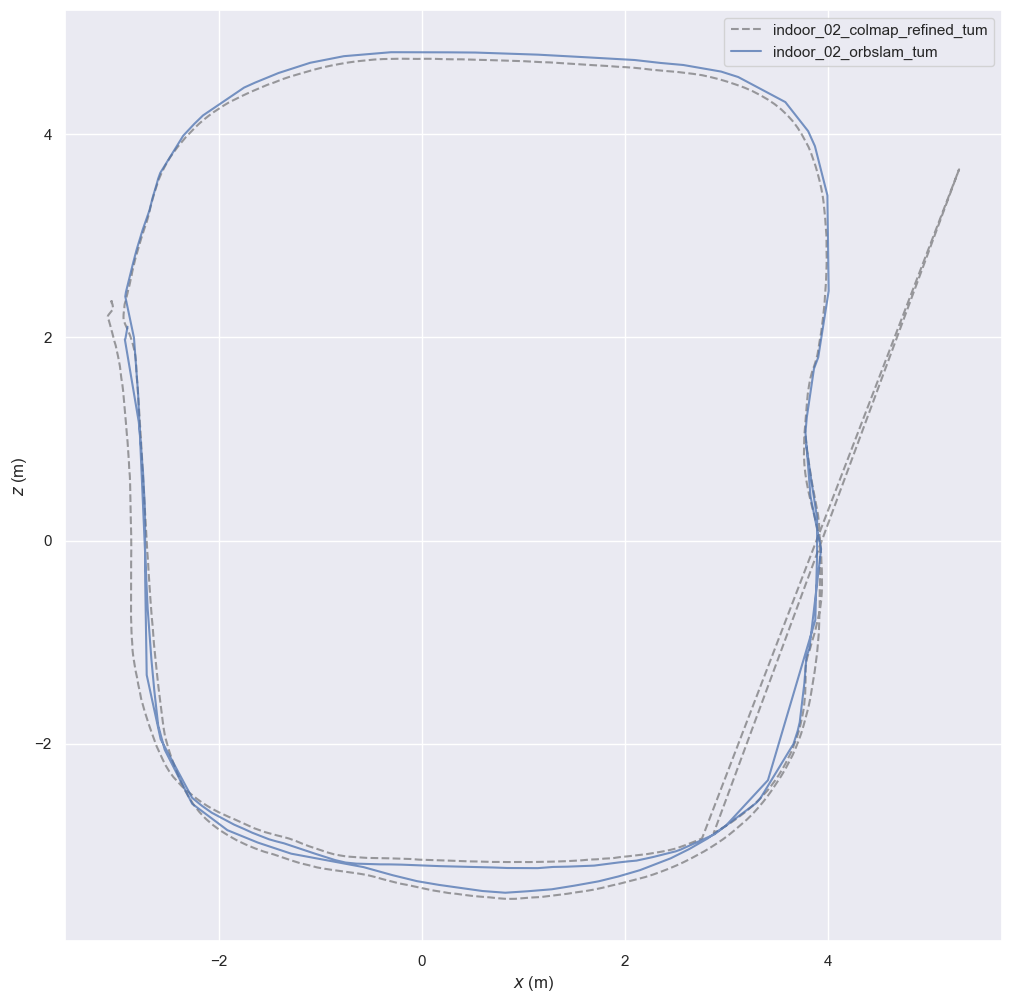
\includegraphics[width=0.24\textwidth]{images/Q2/figures/evo/indoor_02/trajectory_overlay.png}
}
\hfill
\subfloat[EVO APE map.]{
    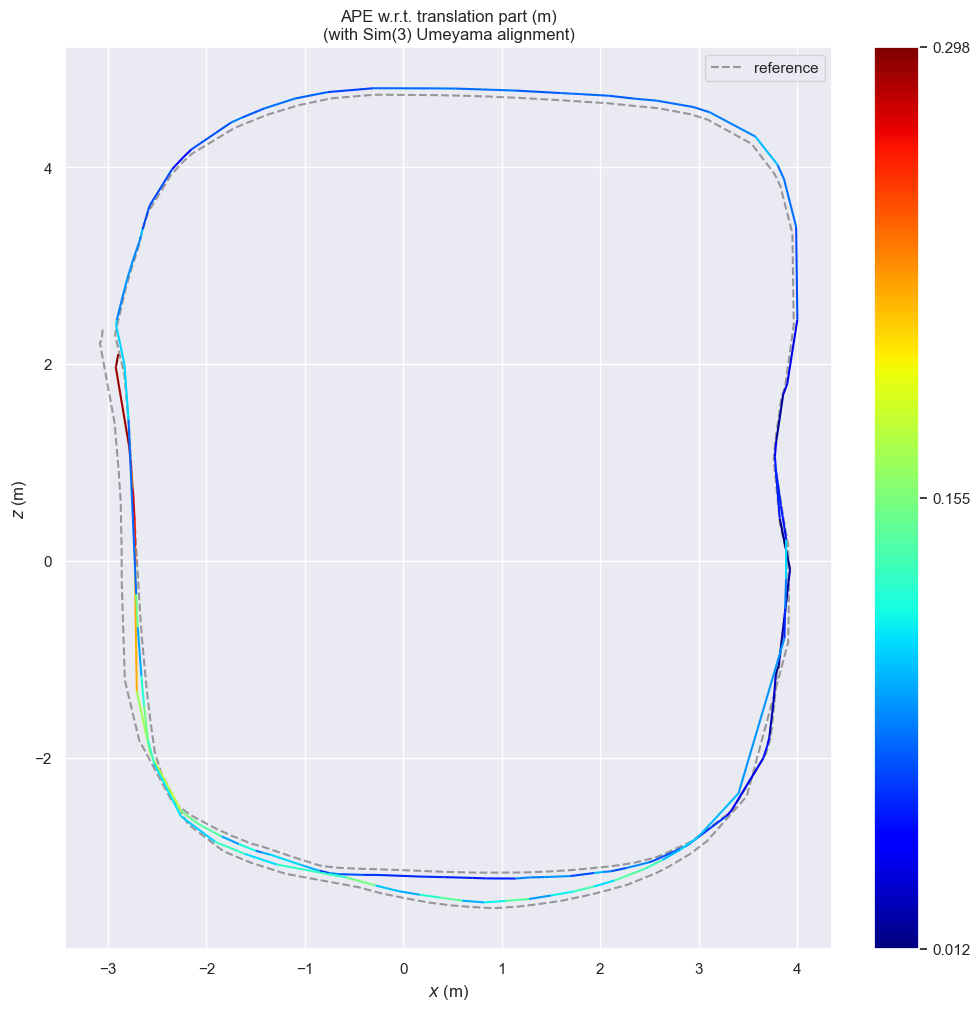
\includegraphics[width=0.24\textwidth]{images/Q2/figures/evo/indoor_02/ape_map.png}
}
\vspace{-1mm}
\caption{Indoor sequence results. COLMAP registered all sampled frames and recovered a loop-like trajectory, but the low-texture walls, glass, carpet, and repeated planar structure make this the harder sequence. ORB-SLAM2 also produced a coherent sparse map, while the EVO comparison shows larger local deviations than in the outdoor sequence.}
\label{fig:q2_indoor_summary}
\end{figure*}

\subsection{Outdoor Sequence}

The outdoor sequence produced a stronger reconstruction. COLMAP again registered all 600 sampled images, but the reconstruction contains more sparse points, more observations, longer tracks, and lower reprojection error than the indoor sequence. This matches the scene content: poles, barriers, signs, facade texture, and building edges provide more repeatable visual features.

Fig.~\ref{fig:q2_outdoor_summary} summarises the outdoor result. Although the sparse point cloud is not dense, the camera route is continuous and geometrically consistent with the acquisition path, which is sufficient for trajectory comparison. ORB-SLAM2 tracked the full outdoor stream and exported 179 keyframes with 12,979 sparse map points. After Sim(3) alignment, the ORB-SLAM2 trajectory closely follows the COLMAP trajectory over most of the route. The outdoor APE RMSE is 0.0298 and the RPE RMSE is 0.0204. Remaining errors occur mainly near turns and the end of the route, where feature overlap decreases and monocular drift becomes more visible.

\begin{figure*}[!t]
\centering
\subfloat[COLMAP sparse top view.]{
    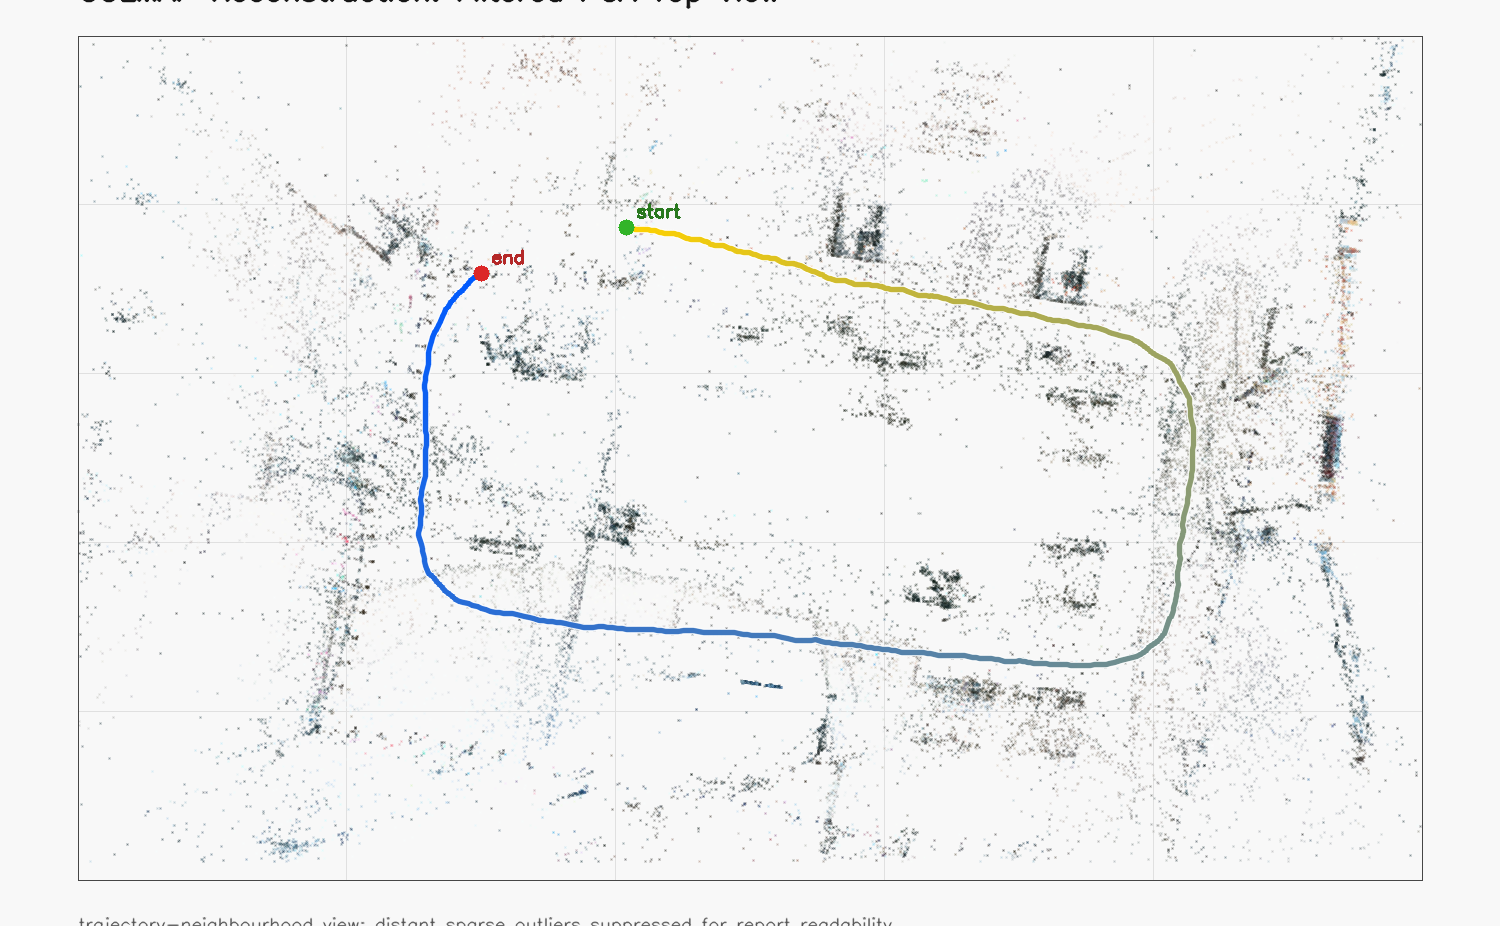
\includegraphics[width=0.24\textwidth]{images/Q2/figures/colmap/outdoor_01/sparse_top_view.png}
}
\hfill
\subfloat[ORB-SLAM2 sparse top view.]{
    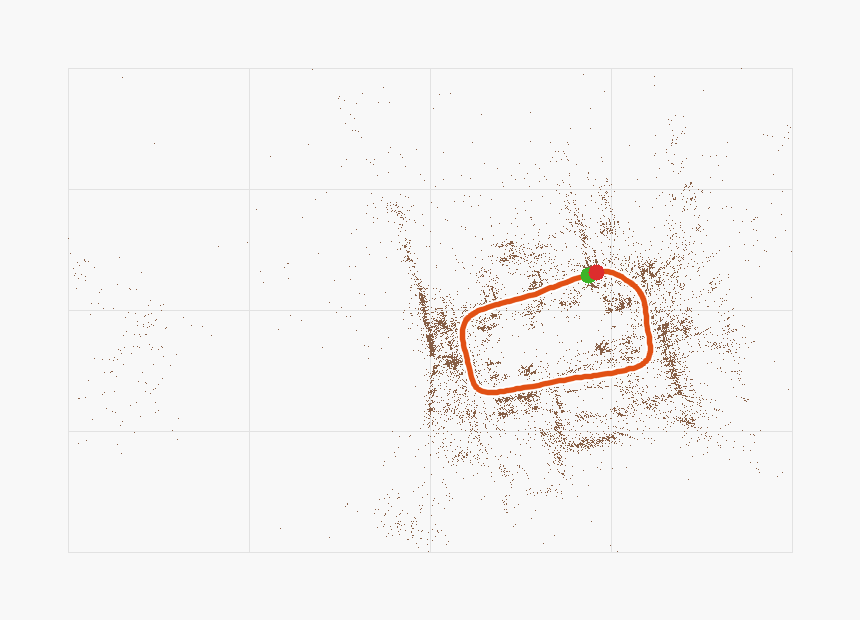
\includegraphics[width=0.24\textwidth]{images/Q2/figures/orbslam/outdoor_01/outdoor_map_top_view.png}
}
\hfill
\subfloat[EVO trajectory overlay.]{
    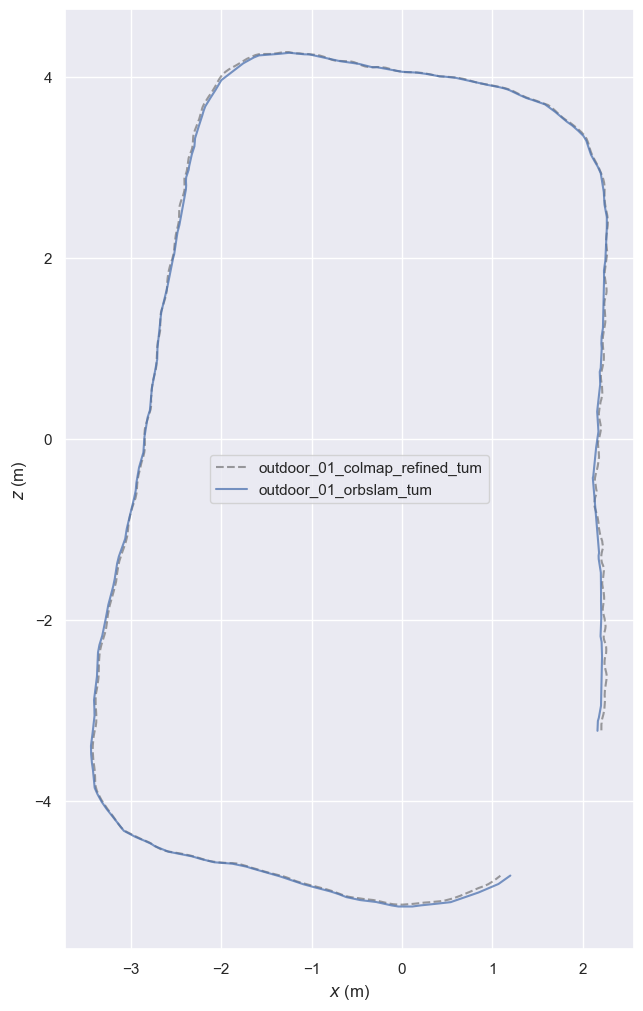
\includegraphics[width=0.24\textwidth]{images/Q2/figures/evo/outdoor_01/trajectory_overlay.png}
}
\hfill
\subfloat[EVO APE map.]{
    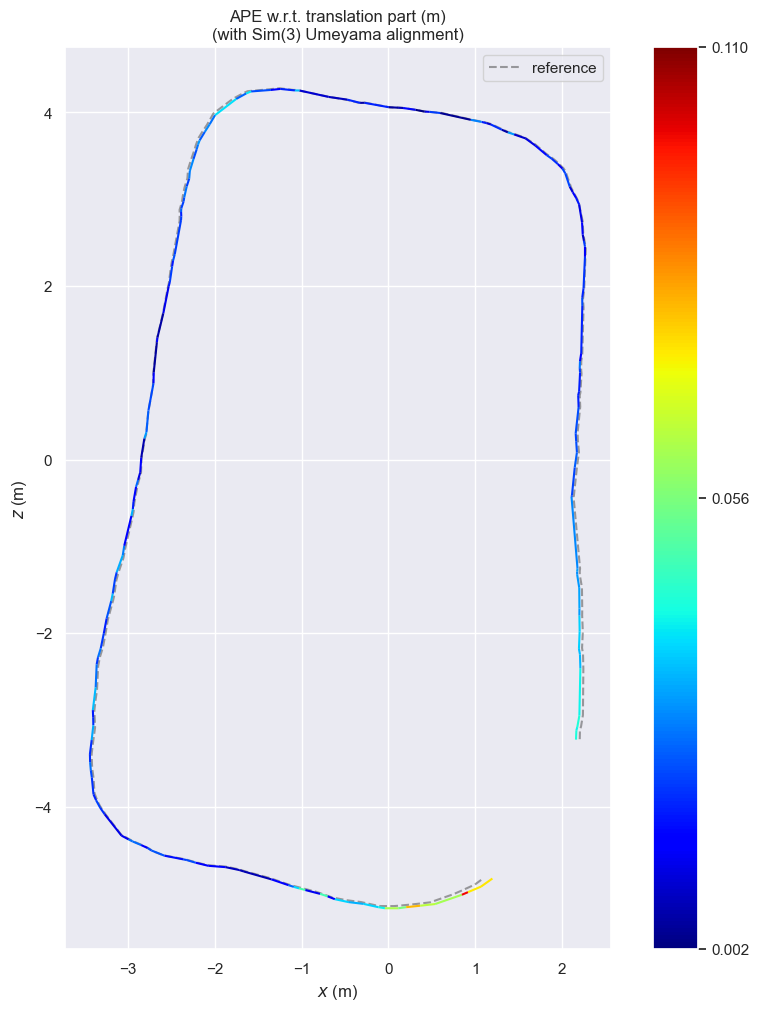
\includegraphics[width=0.24\textwidth]{images/Q2/figures/evo/outdoor_01/ape_map.png}
}
\vspace{-1mm}
\caption{Outdoor sequence results. The outdoor scene provides stronger geometric edges, poles, barriers, signs, and facade texture. This produces longer COLMAP tracks and more stable ORB-SLAM2 tracking. After Sim(3) alignment, the ORB-SLAM2 trajectory closely follows the COLMAP trajectory, with only small local errors near turns and the end of the route.}
\label{fig:q2_outdoor_summary}
\end{figure*}

\subsection{Quantitative Comparison}

Table~\ref{tab:q2_colmap_stats} summarises the COLMAP sparse reconstruction statistics. The outdoor sequence has 41,226 sparse points and a mean track length of 15.70, compared with 31,074 sparse points and 9.70 mean track length indoors. This supports the qualitative observation that the outdoor scene provides stronger and more persistent feature tracks.

\begin{table}[!t]
\caption{COLMAP sparse reconstruction statistics. Units are COLMAP reconstruction units because monocular scale is arbitrary.}
\centering
\footnotesize
\begin{tabular}{lcc}
\toprule
Quantity & Indoor & Outdoor \\
\midrule
Sampled images & 600 & 600 \\
Registered images & 600 & 600 \\
Sparse points & 31,074 & 41,226 \\
Observations & 301,296 & 647,183 \\
Mean track length & 9.70 & 15.70 \\
Mean reproj. error (px) & 0.673 & 0.538 \\
\bottomrule
\end{tabular}
\label{tab:q2_colmap_stats}
\end{table}

Table~\ref{tab:q2_evo_metrics} reports the EVO consistency metrics. These numbers measure agreement with COLMAP rather than absolute metric accuracy. The outdoor sequence has lower APE and RPE values, which is consistent with its sharper frames, stronger edges, more good matches, longer COLMAP tracks, and lower reprojection error.

\begin{table}[!t]
\caption{EVO consistency metrics after timestamp association and Sim(3) alignment to the refined COLMAP trajectory. Since no external ground truth was available, these values measure agreement with COLMAP rather than absolute metric accuracy.}
\centering
\footnotesize
\begin{tabular}{lcc}
\toprule
Metric & Indoor & Outdoor \\
\midrule
Synced ORB poses & 134 & 166 \\
APE RMSE & 0.1221 & 0.0298 \\
APE mean & 0.1045 & 0.0252 \\
APE max & 0.2979 & 0.1104 \\
RPE RMSE & 0.0281 & 0.0204 \\
RPE mean & 0.0229 & 0.0171 \\
RPE max & 0.0723 & 0.0480 \\
\bottomrule
\end{tabular}
\label{tab:q2_evo_metrics}
\end{table}

\subsection{Discussion and Limitations}

The indoor sequence remained valid, but it was harder for both COLMAP and ORB-SLAM2. The main causes were low-texture white walls, glass reflections, repeated planar layout, carpet, and occasional moving people. These factors reduce feature distinctiveness and make feature tracks shorter. ORB-SLAM2 is particularly sensitive to this because it is an online tracker that selects keyframes and map points incrementally.

The outdoor sequence showed closer agreement between ORB-SLAM2 and COLMAP. This should not be interpreted as absolute ground-truth accuracy. Instead, it indicates stronger consistency between two monocular pipelines after Sim(3) alignment. The improvement is explained by sharper frames, stronger geometric edges, more stable feature matches, longer COLMAP tracks, and lower reprojection error.

Several choices were important for stable results. Slow translational motion preserved feature overlap while still providing parallax. Using a single shared camera model in COLMAP avoided per-image intrinsics drift. Sampling every 3rd frame indoors and every 5th frame outdoors kept reconstruction tractable while preserving the full route. Increasing ORB-SLAM2 to 2000 ORB features helped retain enough landmarks in the indoor scene.

The evaluation is limited by the absence of external ground truth. Since both COLMAP and ORB-SLAM2 were used in monocular mode, absolute scale is not directly observable. Sim(3) alignment removes global scale differences, so the evaluation is suitable for comparing trajectory shape and local consistency, but not for claiming true metric accuracy.

The submitted video includes the raw indoor and outdoor streams, screen captures of ORB-SLAM2 reconstructing both scenes, COLMAP sparse reconstruction visualisations, and the EVO trajectory comparison plots. These materials provide supplementary evidence for the reconstruction quality and trajectory consistency discussed in this section.

\FloatBarrier

% ============================================================
\section{LiDAR SLAM with Our Own Sequences}
\label{sec:q3_lidar_slam}

\subsection{Data Collection}

We used three RP-Lidar A2M12 recordings for the LiDAR part: \texttt{indoor\_large\_03}, \texttt{indoor\_small\_01}, and \texttt{outdoor\_02}. The large indoor scene is the same classroom area used for the camera sequence. The small indoor scene is a small meeting room. The outdoor scene is the same general outdoor place as the camera sequence, but the LiDAR route is different. In each run, the LiDAR was carried roughly level, starting from a marked point. The route was walked twice and then returned to the start. The marked loop points were kept for checking the result, not for helping the odometry.

Table~\ref{tab:q3_data_collection} summarises the data. The large classroom gives strong wall and furniture returns. The small room is shorter, but because the path is compact, small errors are easier to see in the final map. The outdoor route is much longer and more open, so it is the hardest case for scan matching.

\begin{table}[!t]
\caption{LiDAR sequences used for Question 3. Each sequence has two manually marked loop completions.}
\centering
\footnotesize
\begin{tabular}{lcrrr}
\toprule
Sequence & Env. & Scans & Time (s) & Rate (Hz) \\
\midrule
\texttt{indoor\_large\_03} & Indoor & 1234 & 96.90 & 12.73 \\
\texttt{indoor\_small\_01} & Indoor & 659 & 60.64 & 10.87 \\
\texttt{outdoor\_02} & Outdoor & 4796 & 407.18 & 11.78 \\
\bottomrule
\end{tabular}
\label{tab:q3_data_collection}
\end{table}

\subsection{Laser Odometry and Mapping}

For the baseline maps, each scan was matched against the growing map to estimate the LiDAR motion. The aligned scans were then combined into point-cloud and occupancy-grid maps. The baseline setting used a 6 m maximum range, all beams, a 0.05 m voxel grid, and every scan.

Figs.~\ref{fig:q3_baseline_large}--\ref{fig:q3_baseline_outdoor} show the baseline maps and trajectories. The large-classroom map is the most stable: the two loops follow a similar shape and the final drift is 0.886 m. The small-room map is compact, but the second loop is less well aligned with the first, giving 3.586 m drift. The outdoor route is much longer, and the trajectory is visibly stretched, with 7.000 m final drift. This shows why the outdoor run is the hardest case for odometry alone.

\begin{figure}[!htbp]
\centering
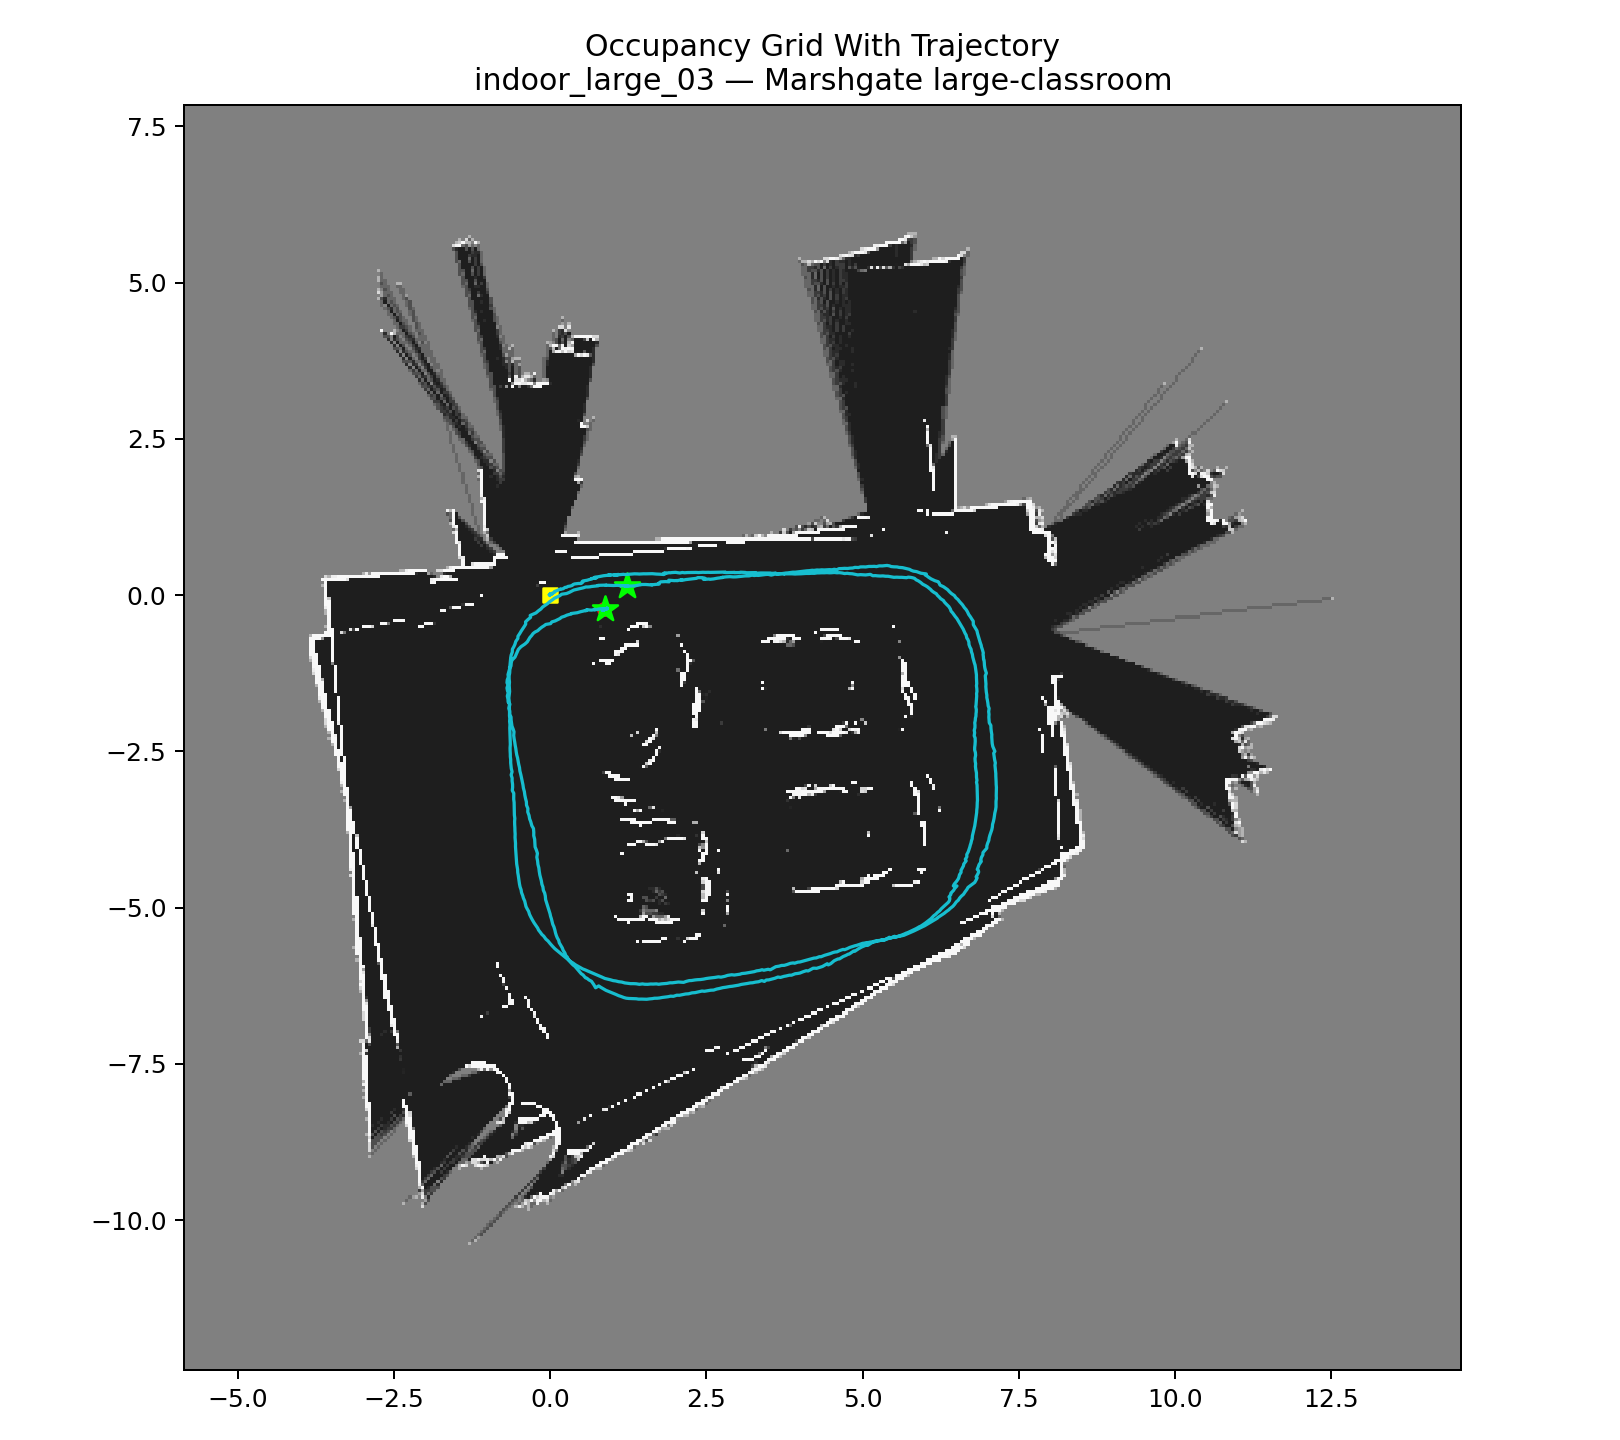
\includegraphics[width=\columnwidth]{images/Q3/baseline_indoor_large.png}
\caption{Baseline large-classroom map. The two loops close fairly well and the main walls stay mostly aligned.}
\label{fig:q3_baseline_large}
\end{figure}

\begin{figure}[!htbp]
\centering
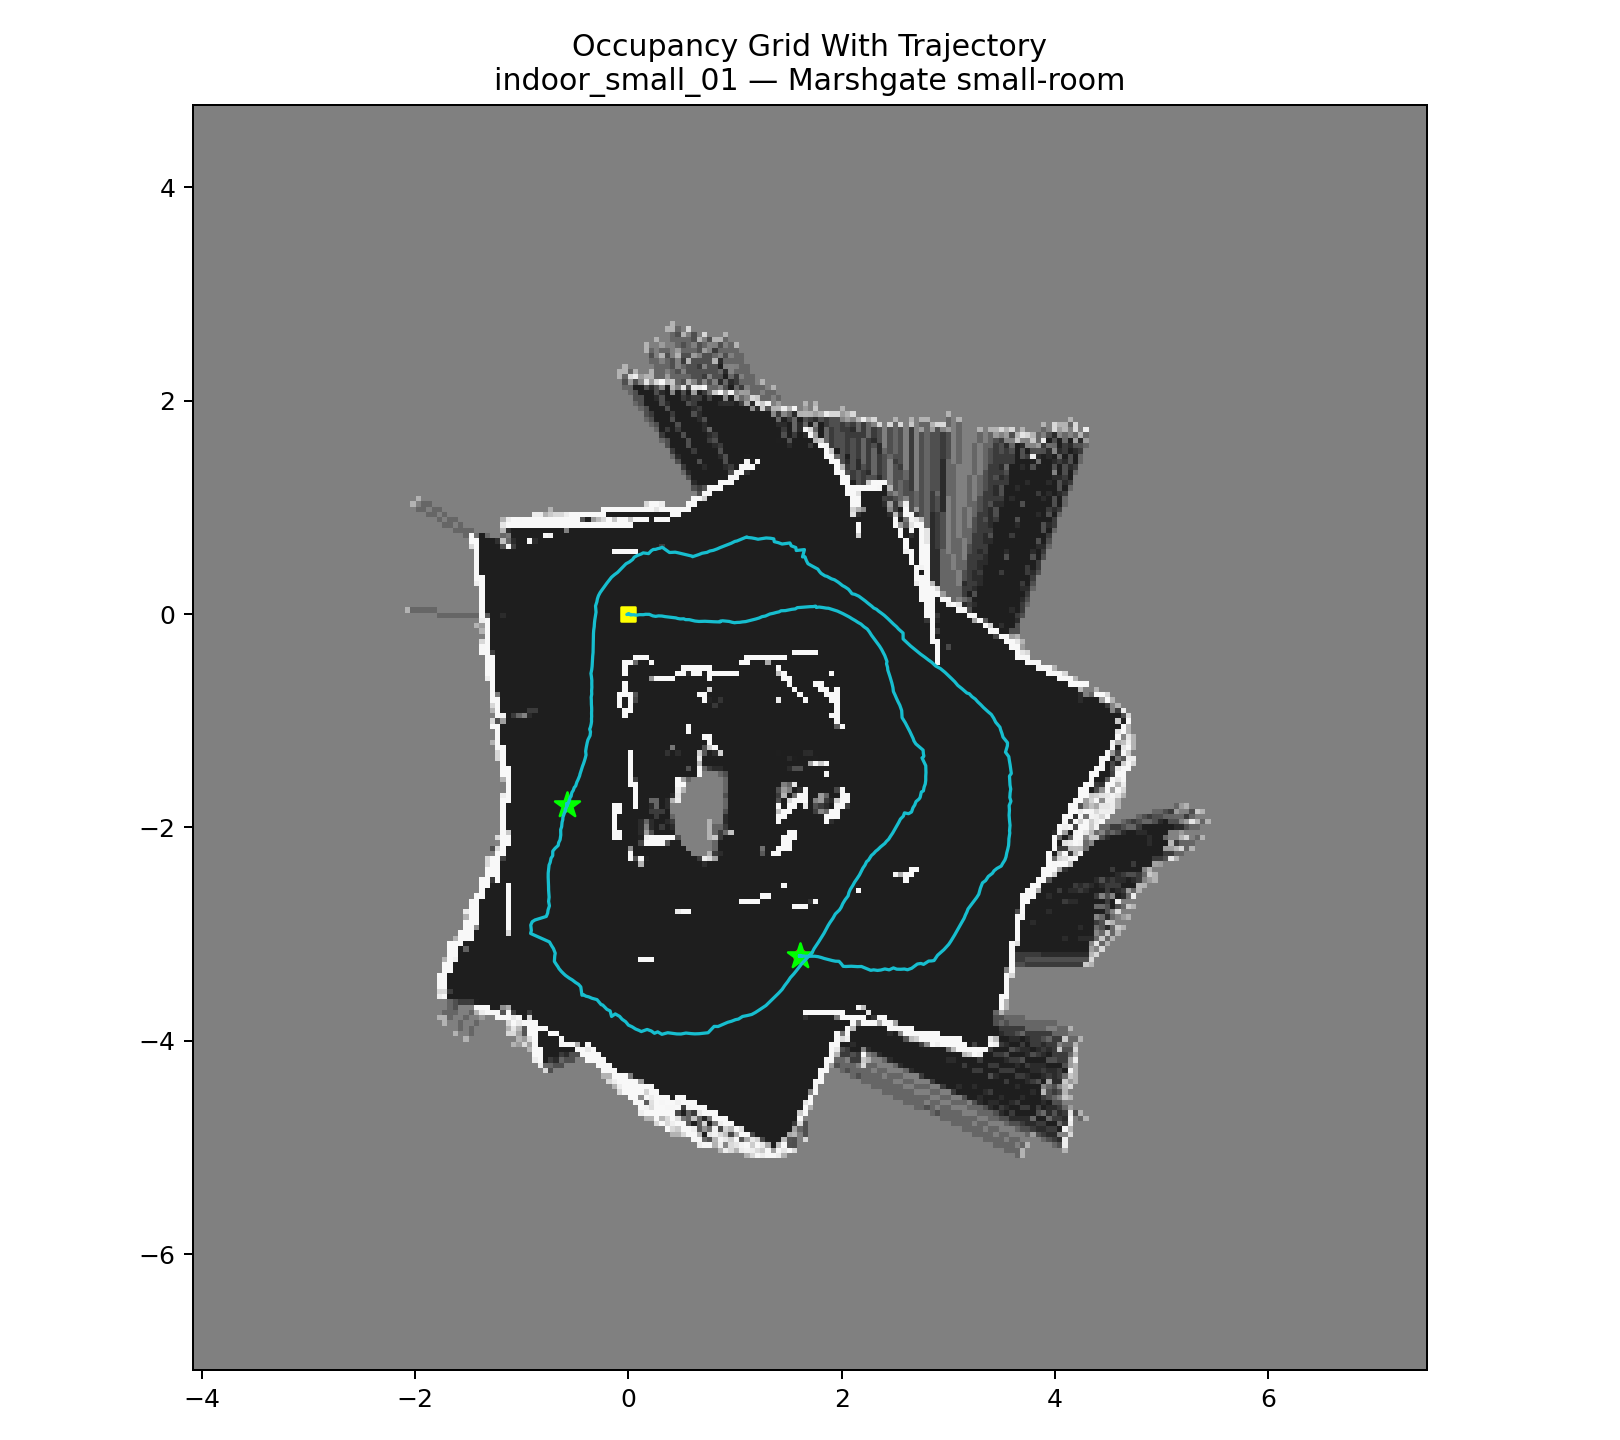
\includegraphics[width=\columnwidth]{images/Q3/baseline_indoor_small.png}
\caption{Baseline small-room map. The compact route makes the second-loop drift easier to see.}
\label{fig:q3_baseline_small}
\end{figure}

\begin{figure}[!htbp]
\centering
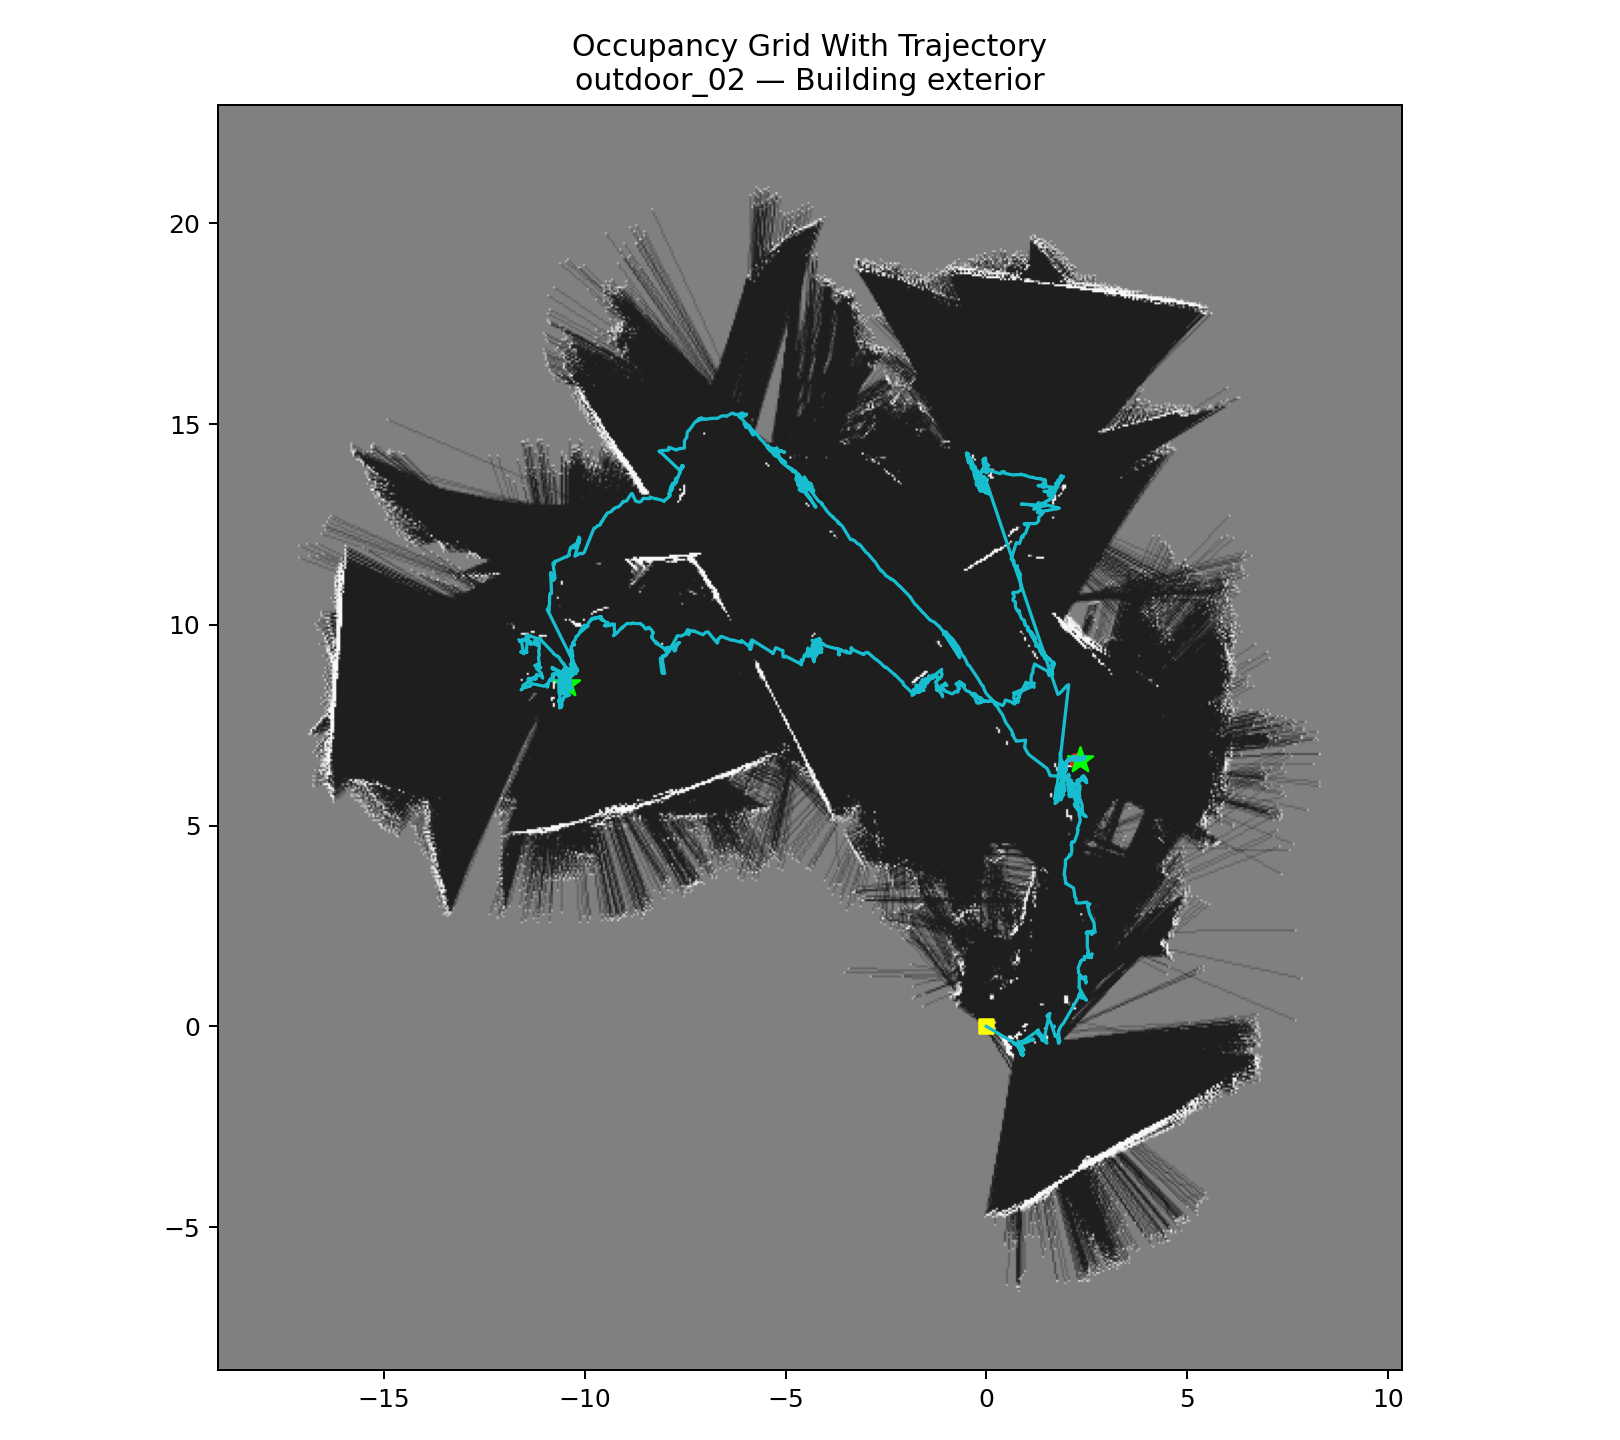
\includegraphics[width=\columnwidth]{images/Q3/baseline_outdoor.png}
\caption{Baseline outdoor map. The longer, more open route gives the largest drift.}
\label{fig:q3_baseline_outdoor}
\end{figure}

\subsection{Parameter Analysis}

The coursework asks us to test four parameters: maximum range, angular resolution, voxel grid size, and scan rate. Table~\ref{tab:q3_parameter_summary} lists the final drift for the main settings. The main result is that there is no single best setting for every place. The useful amount of scan detail changes with the size and structure of the environment.

\begin{table}[!htbp]
\caption{Parameter-study final drift results in metres.}
\centering
\scriptsize
\setlength{\tabcolsep}{3pt}
\begin{tabular}{llccc}
\toprule
Study & Setting & Large & Small & Outdoor \\
\midrule
Range & 6 m & 0.886 & 3.586 & 7.000 \\
Range & 12 m & 0.494 & 2.301 & 18.183 \\
Beams & Full & 0.886 & 3.586 & 7.000 \\
Beams & 1/2 & 0.451 & 4.782 & 9.203 \\
Beams & 1/3 & 0.852 & 2.258 & 7.875 \\
Voxel & 0.05 m & 0.886 & 3.586 & 7.000 \\
Voxel & 0.10 m & 0.886 & 3.674 & 2251.157 \\
Scans & All & 0.886 & 3.586 & 7.000 \\
Scans & 1/2 & 0.915 & 0.608 & 2.820 \\
Scans & 1/3 & 0.687 & 1.978 & 3.708 \\
\bottomrule
\end{tabular}
\label{tab:q3_parameter_summary}
\end{table}

Maximum range behaves differently indoors and outdoors. In Fig.~\ref{fig:q3_param_range}, increasing the range from 6 m to 12 m improves both indoor sequences because the scan contains more walls and room boundaries. Outdoors, the same change makes the result worse, increasing drift from 7.000 m to 18.183 m, because distant returns are less reliable for matching.

\begin{figure}[!htbp]
\centering
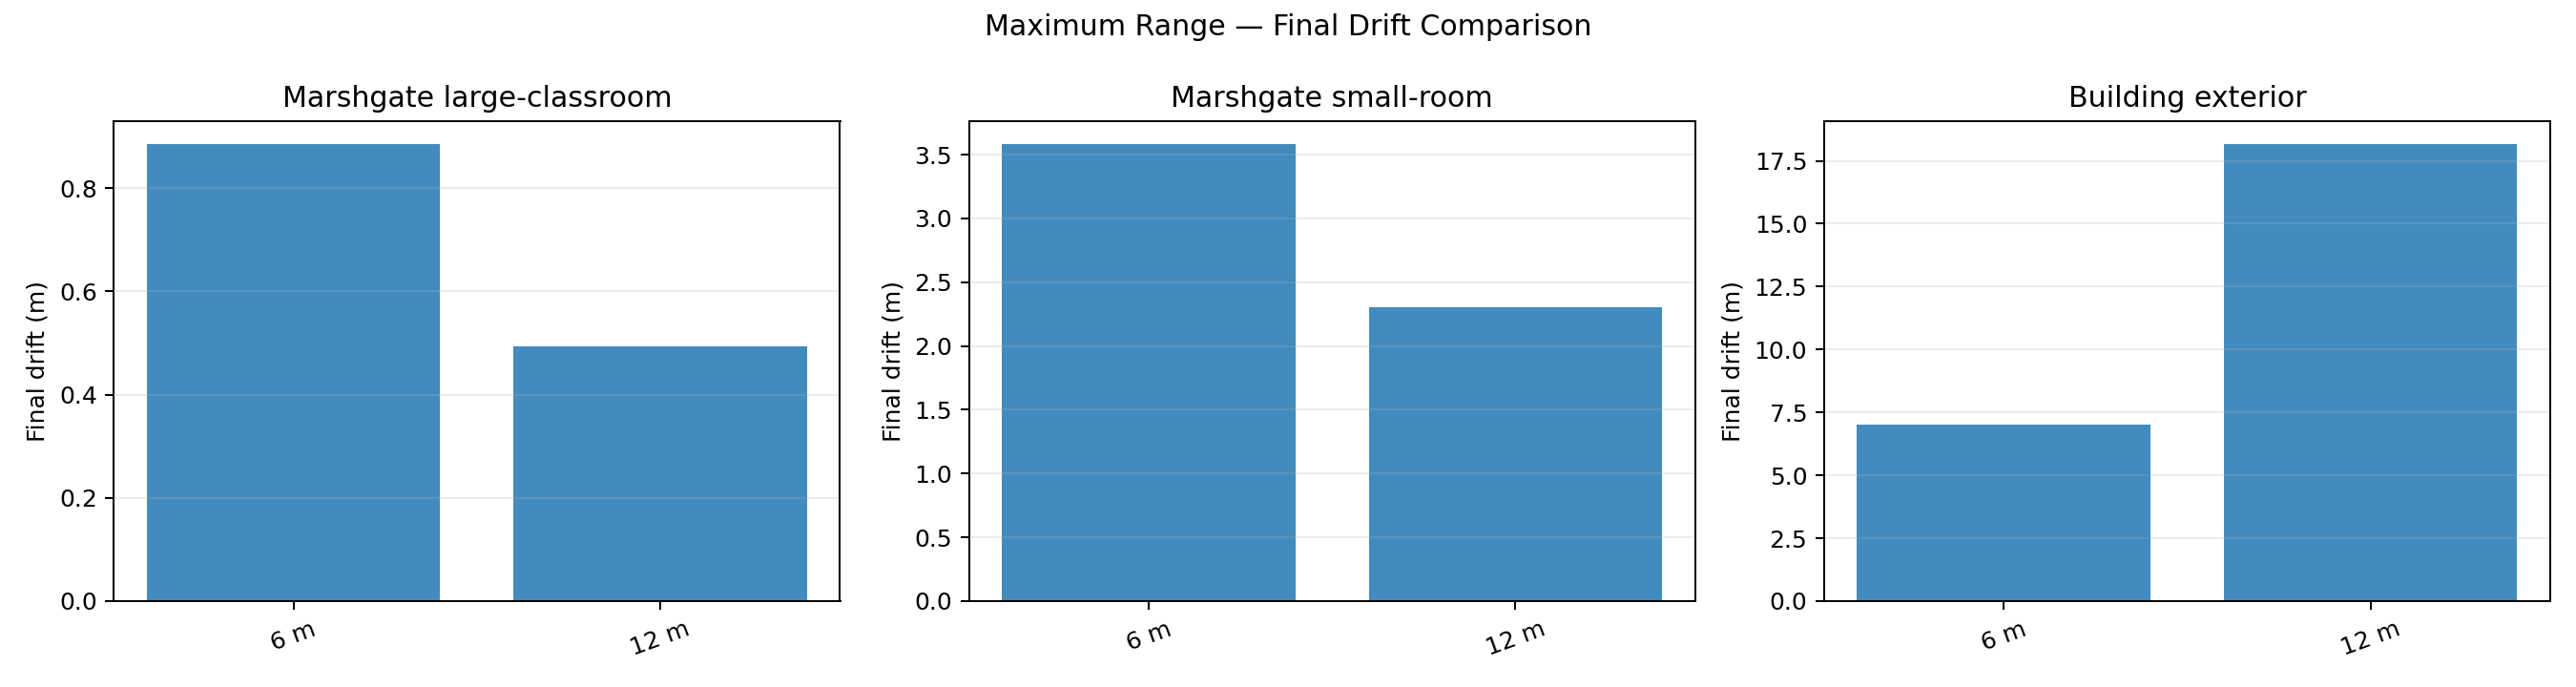
\includegraphics[width=\columnwidth]{images/Q3/param_max_range.png}
\caption{Maximum-range experiment. The 12 m range helps indoors but hurts outdoors because distant returns are less reliable.}
\label{fig:q3_param_range}
\end{figure}

Angular downsampling also depends on the scene. Fig.~\ref{fig:q3_param_angular} shows that using every 2nd beam gives the lowest drift in the large classroom, while every 3rd beam works best in the small room. Outdoors, the full scan is still best because the route already has less nearby structure, so removing beams loses useful information.

\begin{figure}[!htbp]
\centering
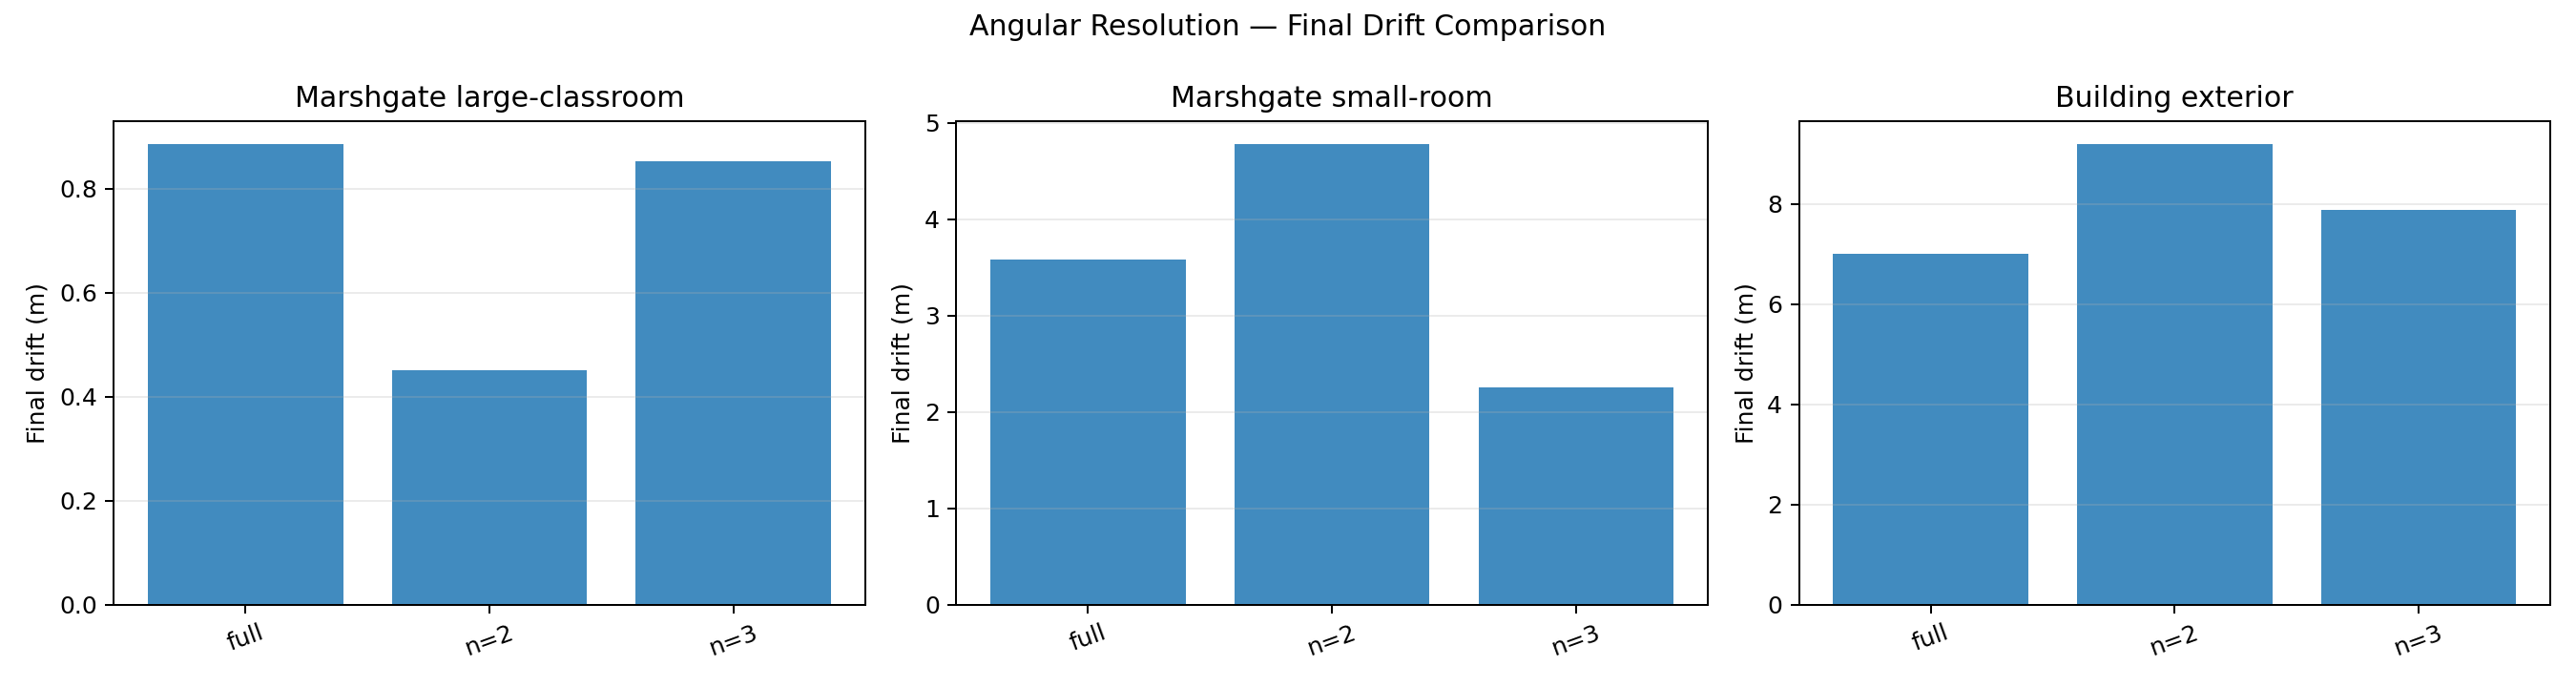
\includegraphics[width=\columnwidth]{images/Q3/param_angular_resolution.png}
\caption{Angular-resolution experiment. Beam downsampling can help indoors, but the outdoor route needs the full scan.}
\label{fig:q3_param_angular}
\end{figure}

The voxel-grid test gives the clearest failure case. A 0.05 m voxel size works on all three sequences, but a 0.10 m grid removes too much detail outdoors. In Fig.~\ref{fig:q3_param_voxel}, the trajectory becomes a long artificial line and the map no longer matches the real route. Because of this, the final runs use the 0.05 m setting.

\begin{figure}[!htbp]
\centering
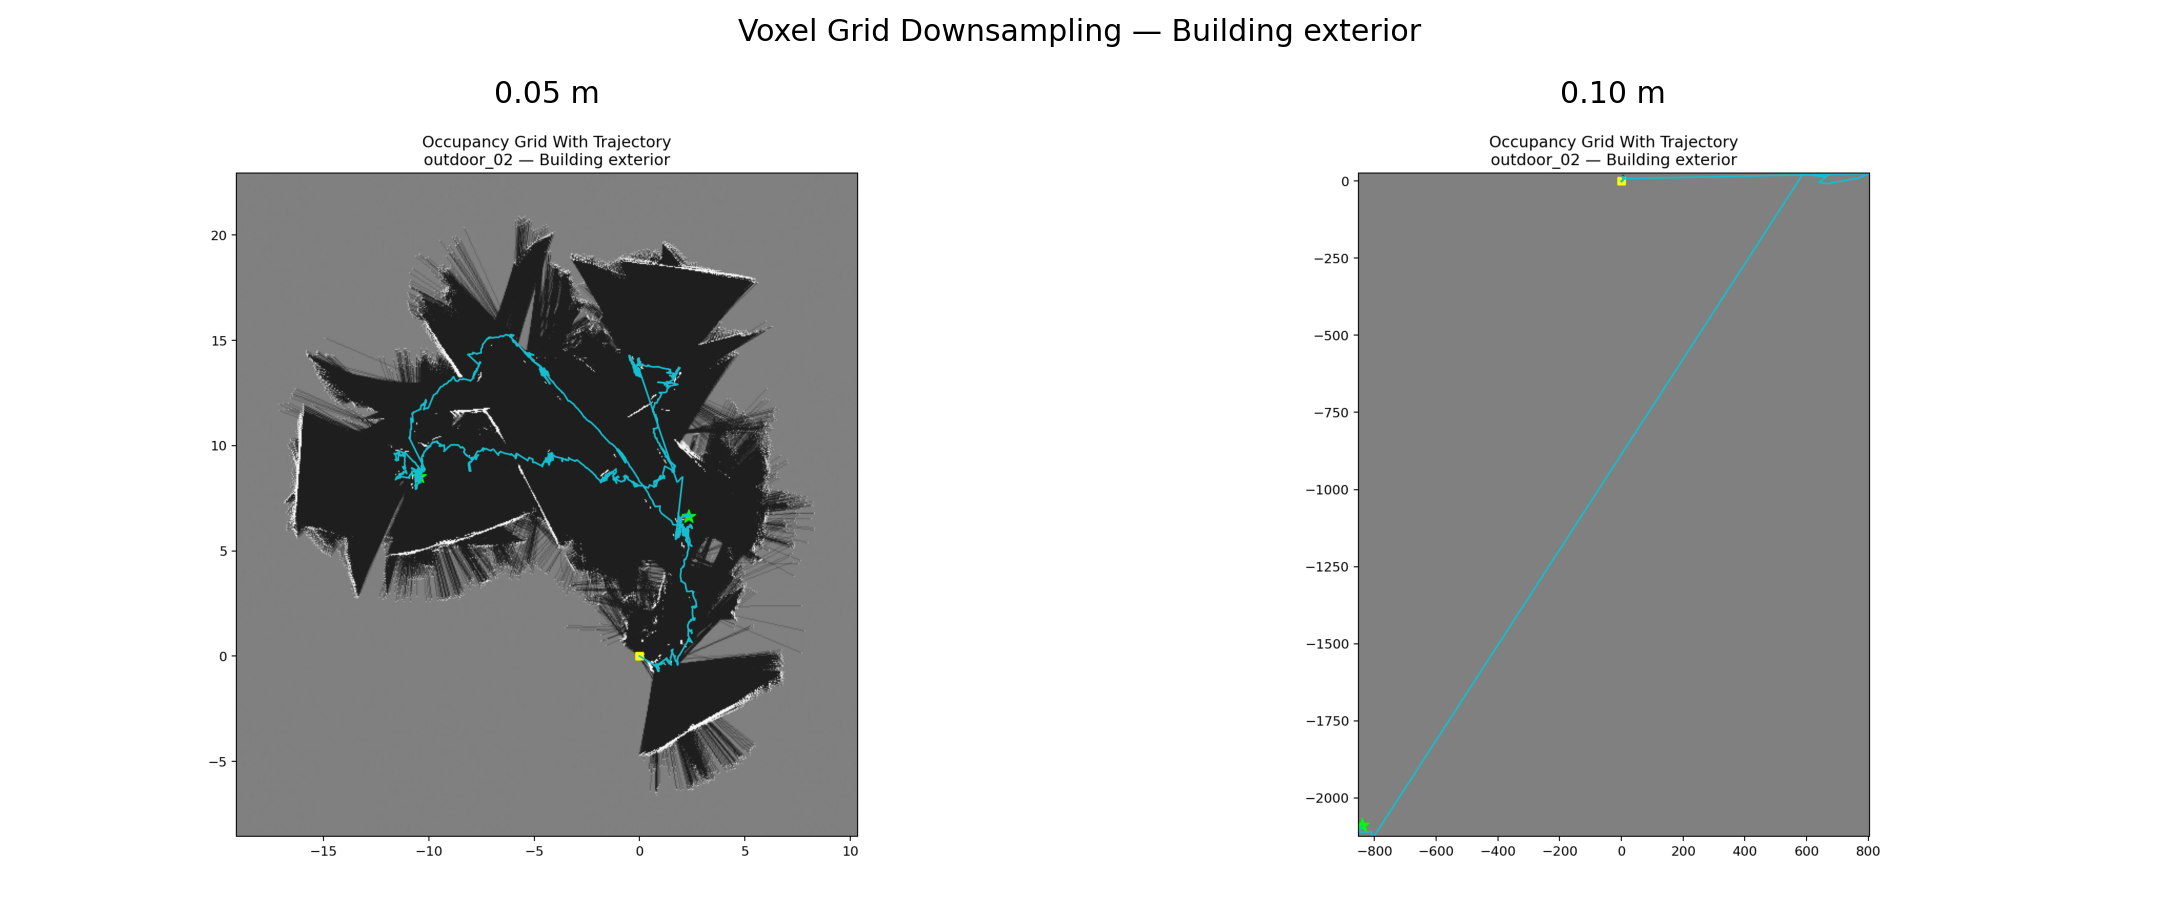
\includegraphics[width=\columnwidth]{images/Q3/param_voxel_outdoor.png}
\caption{Outdoor voxel-grid result. The 0.05 m grid keeps enough detail, while the 0.10 m grid is too coarse and fails badly.}
\label{fig:q3_param_voxel}
\end{figure}

Reducing the scan rate did not simply make the result worse. Fig.~\ref{fig:q3_param_scan_rate} shows that using every 2nd scan improves the small-room and outdoor drift, while every 3rd scan is best for the large classroom. For these recordings, skipping some scans may reduce small local matching errors. This should not be treated as a general rule, since the best scan rate also depends on walking speed and scene layout.

\begin{figure}[!htbp]
\centering
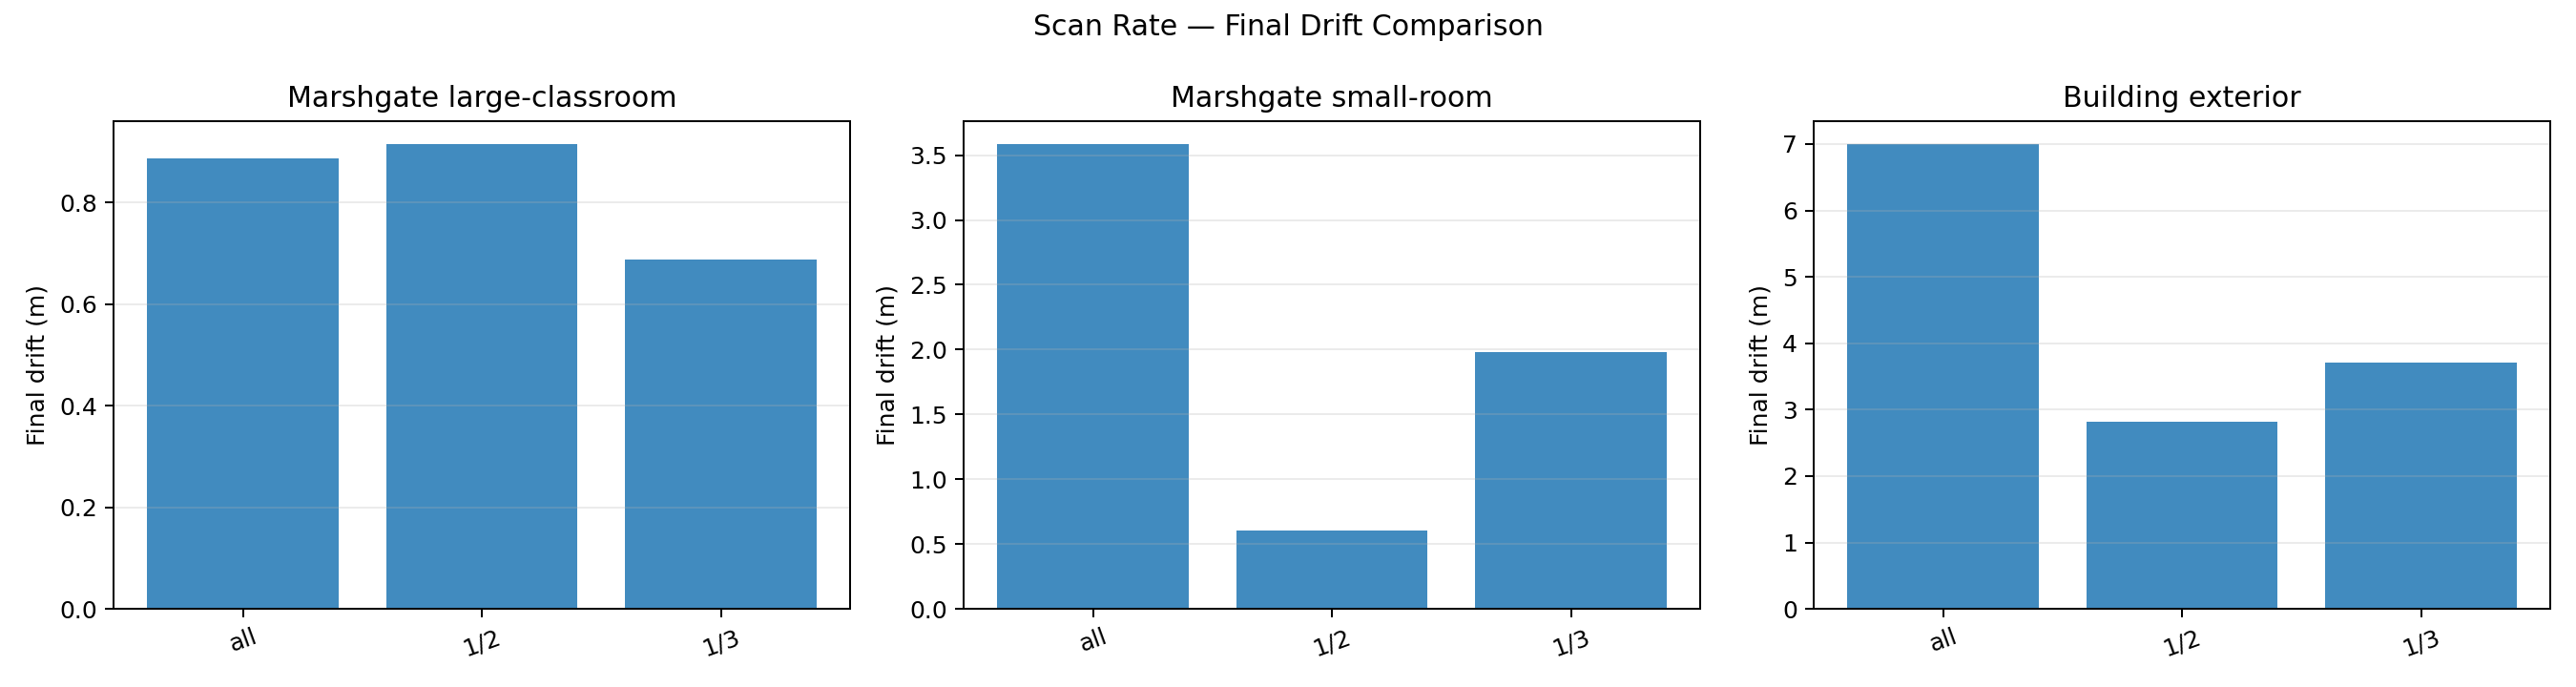
\includegraphics[width=\columnwidth]{images/Q3/param_scan_rate.png}
\caption{Scan-rate experiment. Skipping scans helps some recordings here, but the best choice depends on the environment.}
\label{fig:q3_param_scan_rate}
\end{figure}

\subsection{Loop Closure Detection}

Loop closure looks for places that the LiDAR has visited before. The detector first removes candidates that are too close in time or distance. It then checks scan similarity, tests whether the scans align well, and removes duplicate matches. The final set keeps both local revisits along the path and anchor loops that connect the second pass back to the start area.

Figs.~\ref{fig:q3_loop_large}--\ref{fig:q3_loop_outdoor} show the accepted loop closures. The large classroom has 7 accepted loops and detects both manual loop markers. The small room has 4 accepted loops and detects one of the two markers. The outdoor route has 12 accepted loops, so the detector does find repeated places, but neither manual marker is matched directly. This makes the outdoor marker comparison weaker, even though useful loop closures are still found.

\begin{figure}[!htbp]
\centering
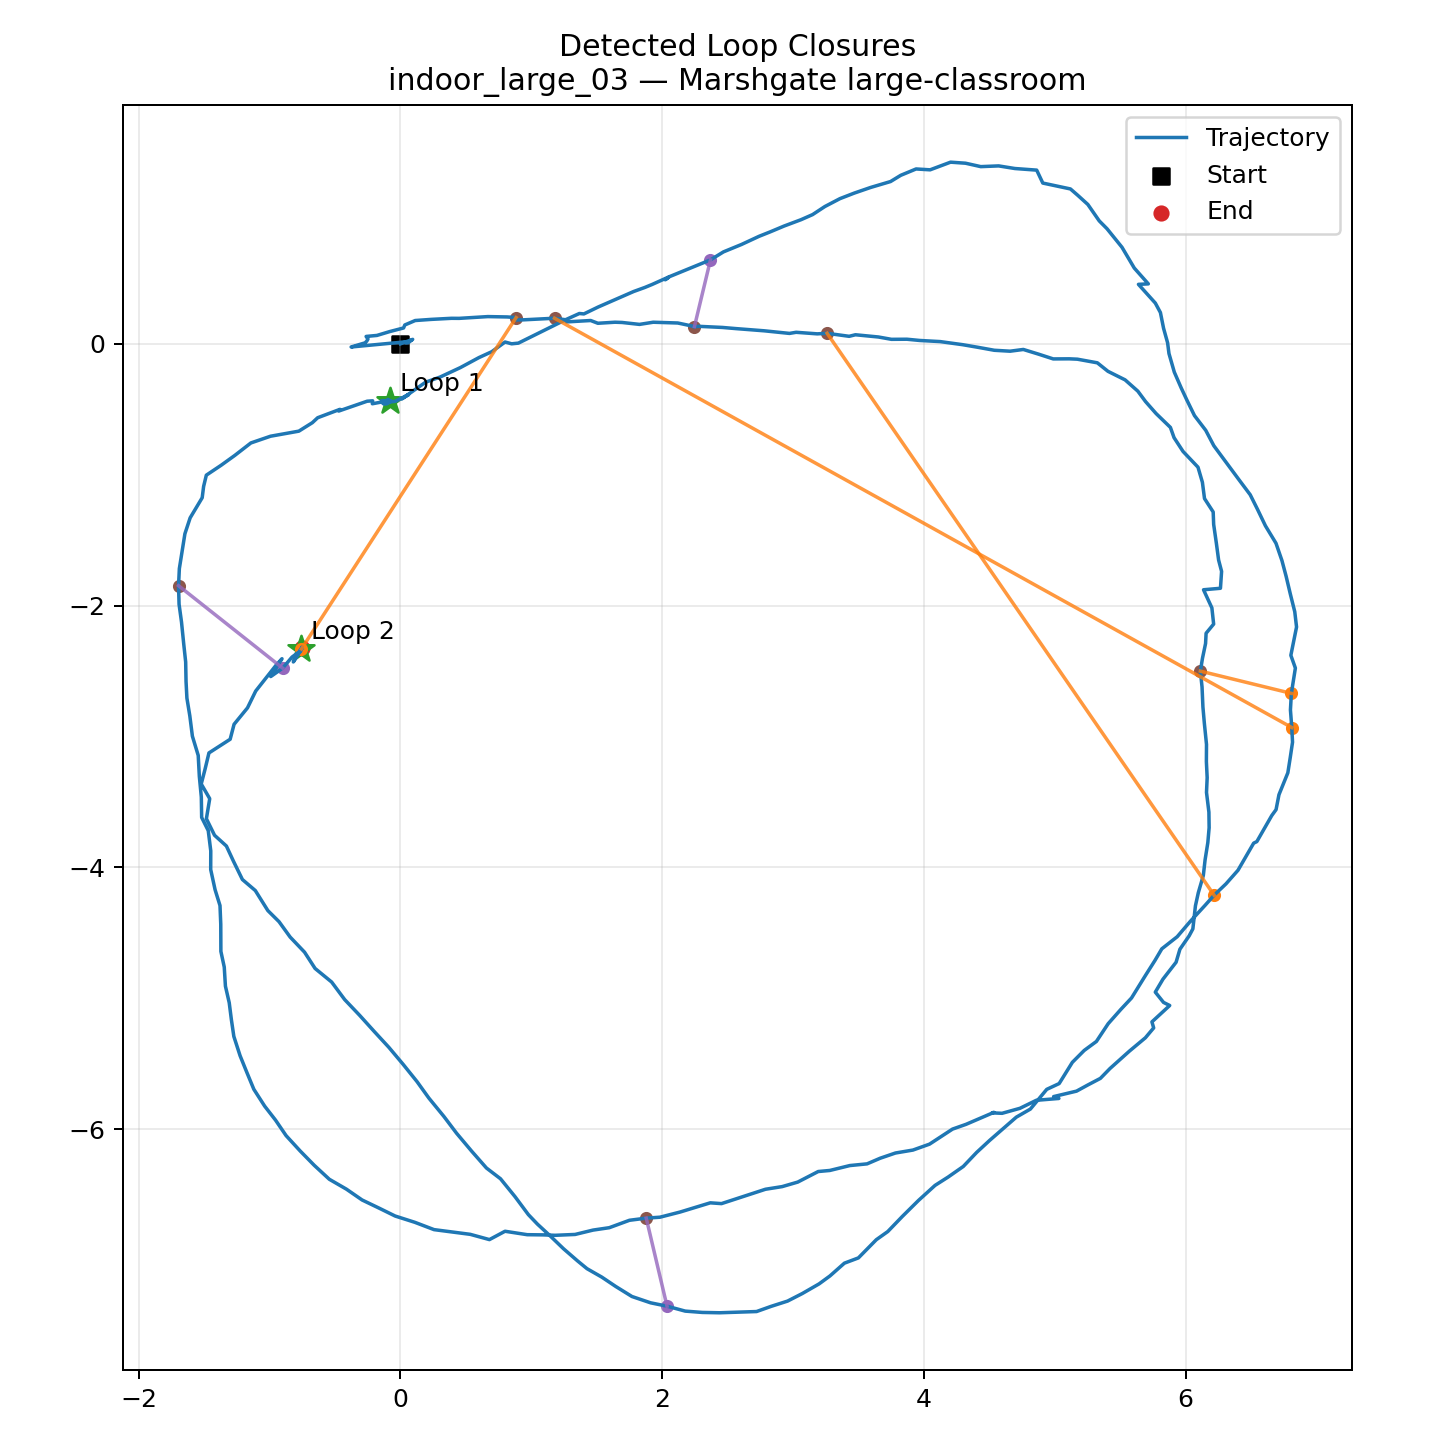
\includegraphics[width=\columnwidth]{images/Q3/loop_indoor_large.png}
\caption{Loop closures in the large indoor sequence. Both manual loop markers are found.}
\label{fig:q3_loop_large}
\end{figure}

\begin{figure}[!htbp]
\centering
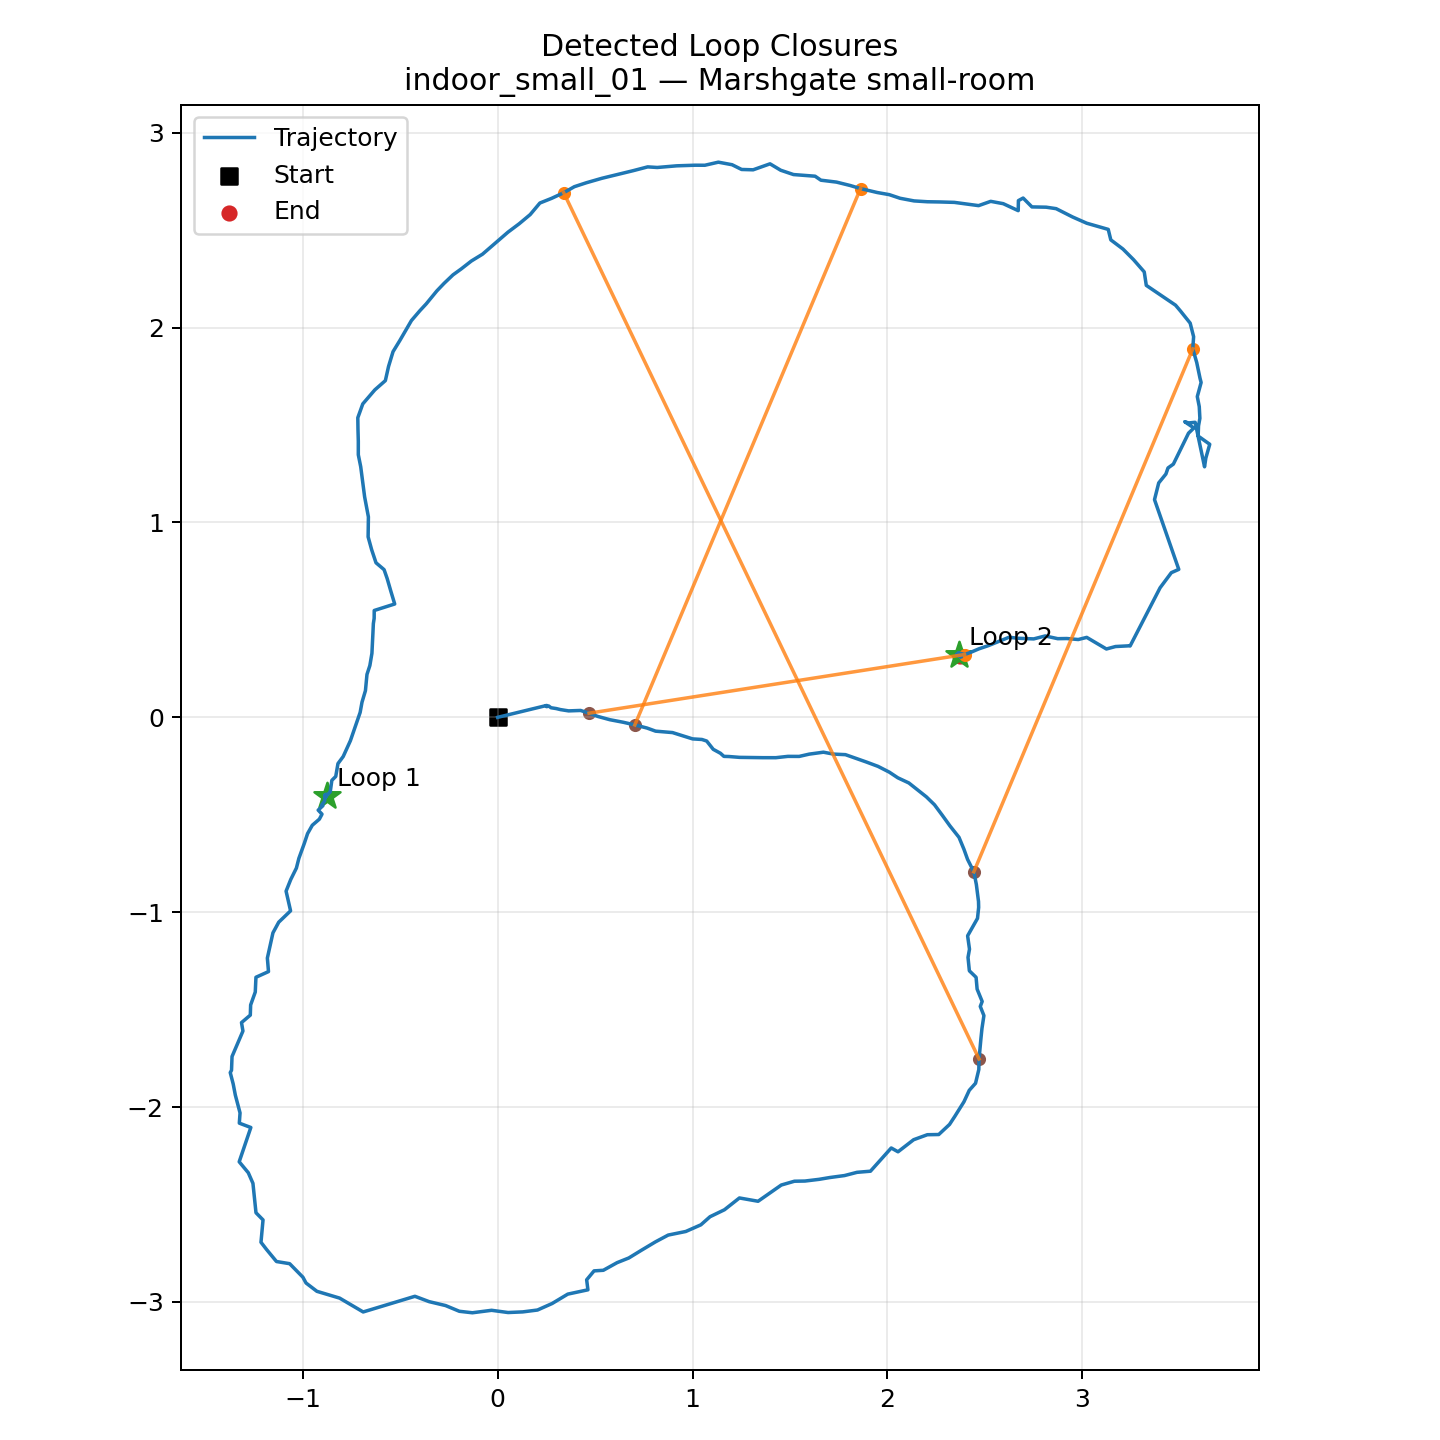
\includegraphics[width=\columnwidth]{images/Q3/loop_indoor_small.png}
\caption{Loop closures in the small indoor sequence. One of the two manual loop markers is found.}
\label{fig:q3_loop_small}
\end{figure}

\begin{figure}[!htbp]
\centering
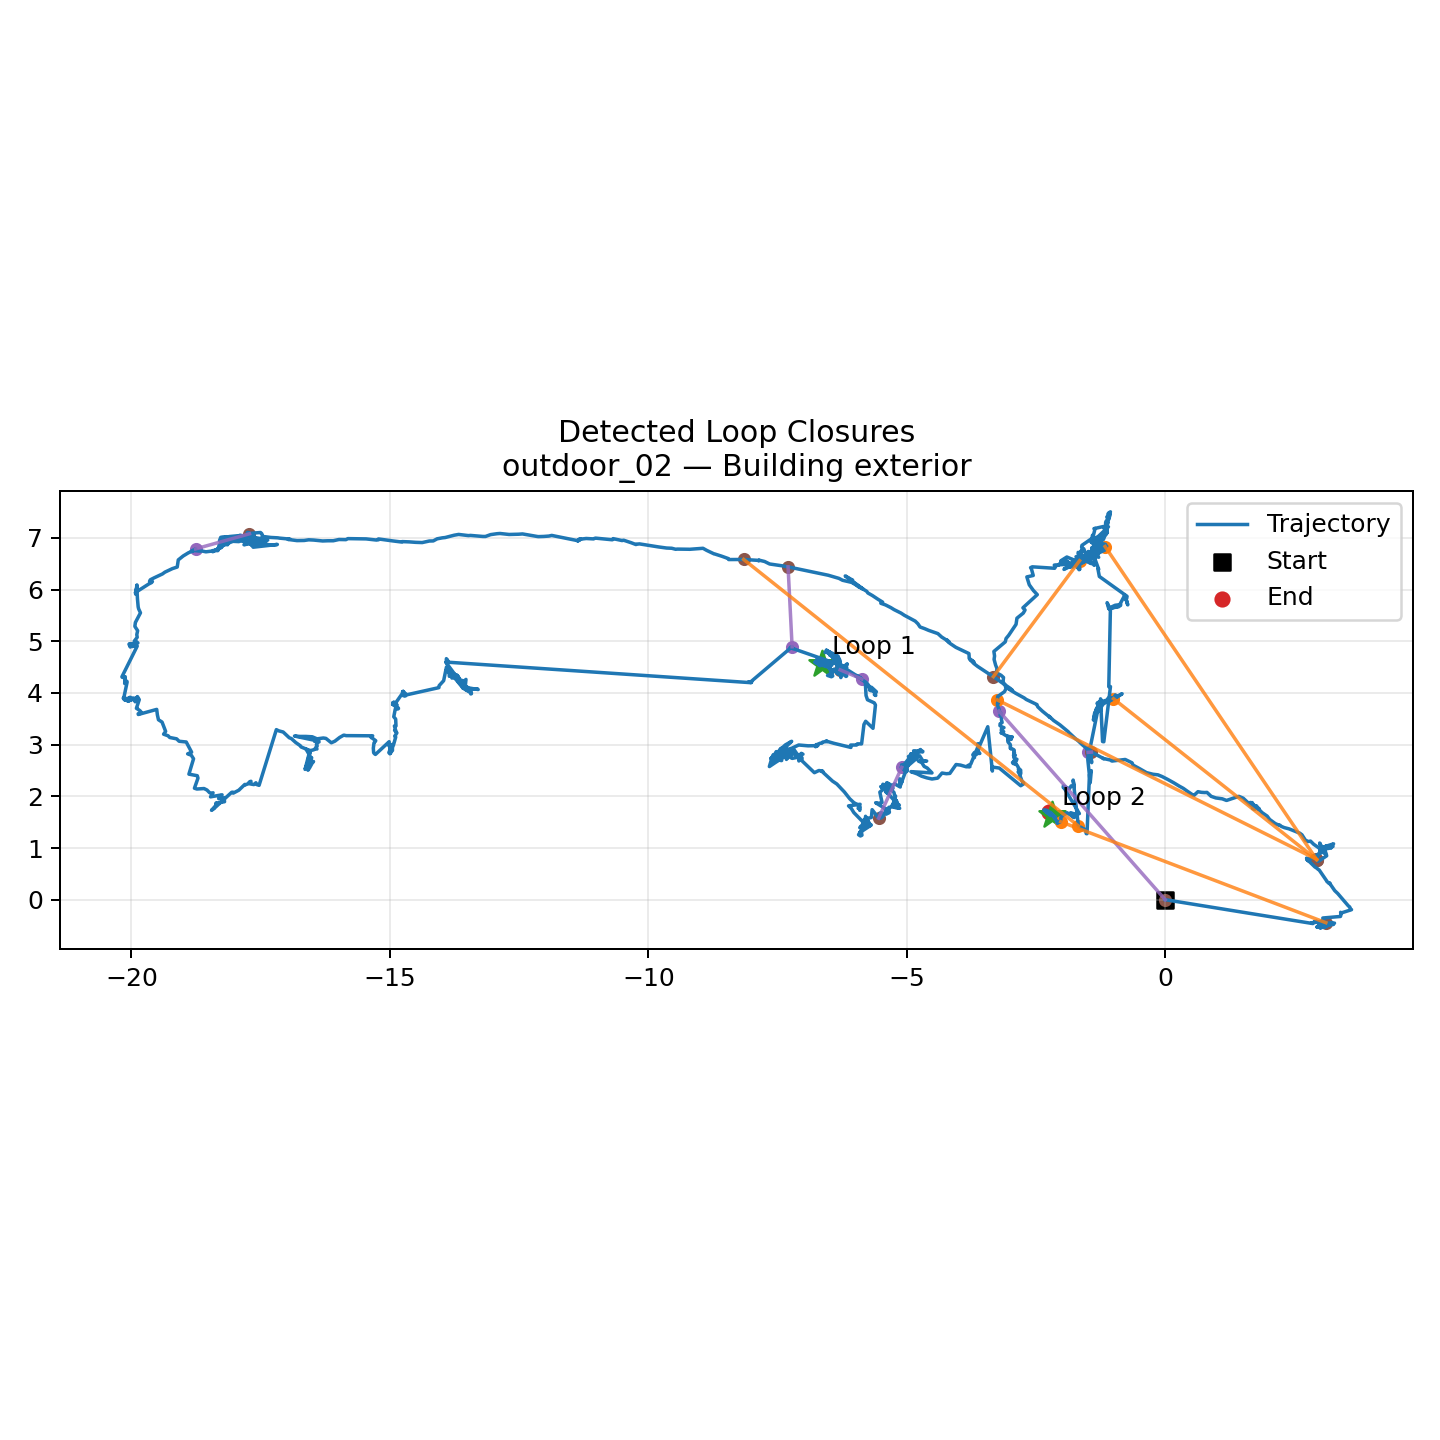
\includegraphics[width=\columnwidth]{images/Q3/loop_outdoor.png}
\caption{Loop closures in the outdoor sequence. Revisited places are found, but neither manual marker is directly matched.}
\label{fig:q3_loop_outdoor}
\end{figure}

\FloatBarrier

\subsection{Factor Graph Optimisation}

The final stage uses a pose graph to correct the trajectory. Consecutive poses are linked by odometry, and accepted revisits are linked by loop-closure edges. We tested several loop-edge choices and selected the ones that closed the route well without bending the map too much. Table~\ref{tab:q3_loop_optimization} summarises the final results.

\begin{table}[!htbp]
\caption{Loop-closure and optimisation summary. Closure error is the distance between the start and final pose.}
\centering
\scriptsize
\setlength{\tabcolsep}{2pt}
\begin{tabular}{lcccc}
\toprule
Sequence & Loops & Hits & Edges & Error (m) \\
\midrule
Large indoor & 7 & 2/2 & 1 & 2.443$\rightarrow$0.898 \\
Small indoor & 4 & 1/2 & 1 & 2.395$\rightarrow$0.546 \\
Outdoor & 12 & 0/2 & 2 & 2.820$\rightarrow$0.817 \\
\bottomrule
\end{tabular}
\label{tab:q3_loop_optimization}
\end{table}

Figs.~\ref{fig:q3_optim_large} and \ref{fig:q3_optim_small} show the two indoor optimisation results. In both cases, one strong anchor loop is enough to bring the final pose close to the start. The large-classroom error is reduced from 2.443 m to 0.898 m, and the small-room error is reduced from 2.395 m to 0.546 m.

\begin{figure}[!htbp]
\centering
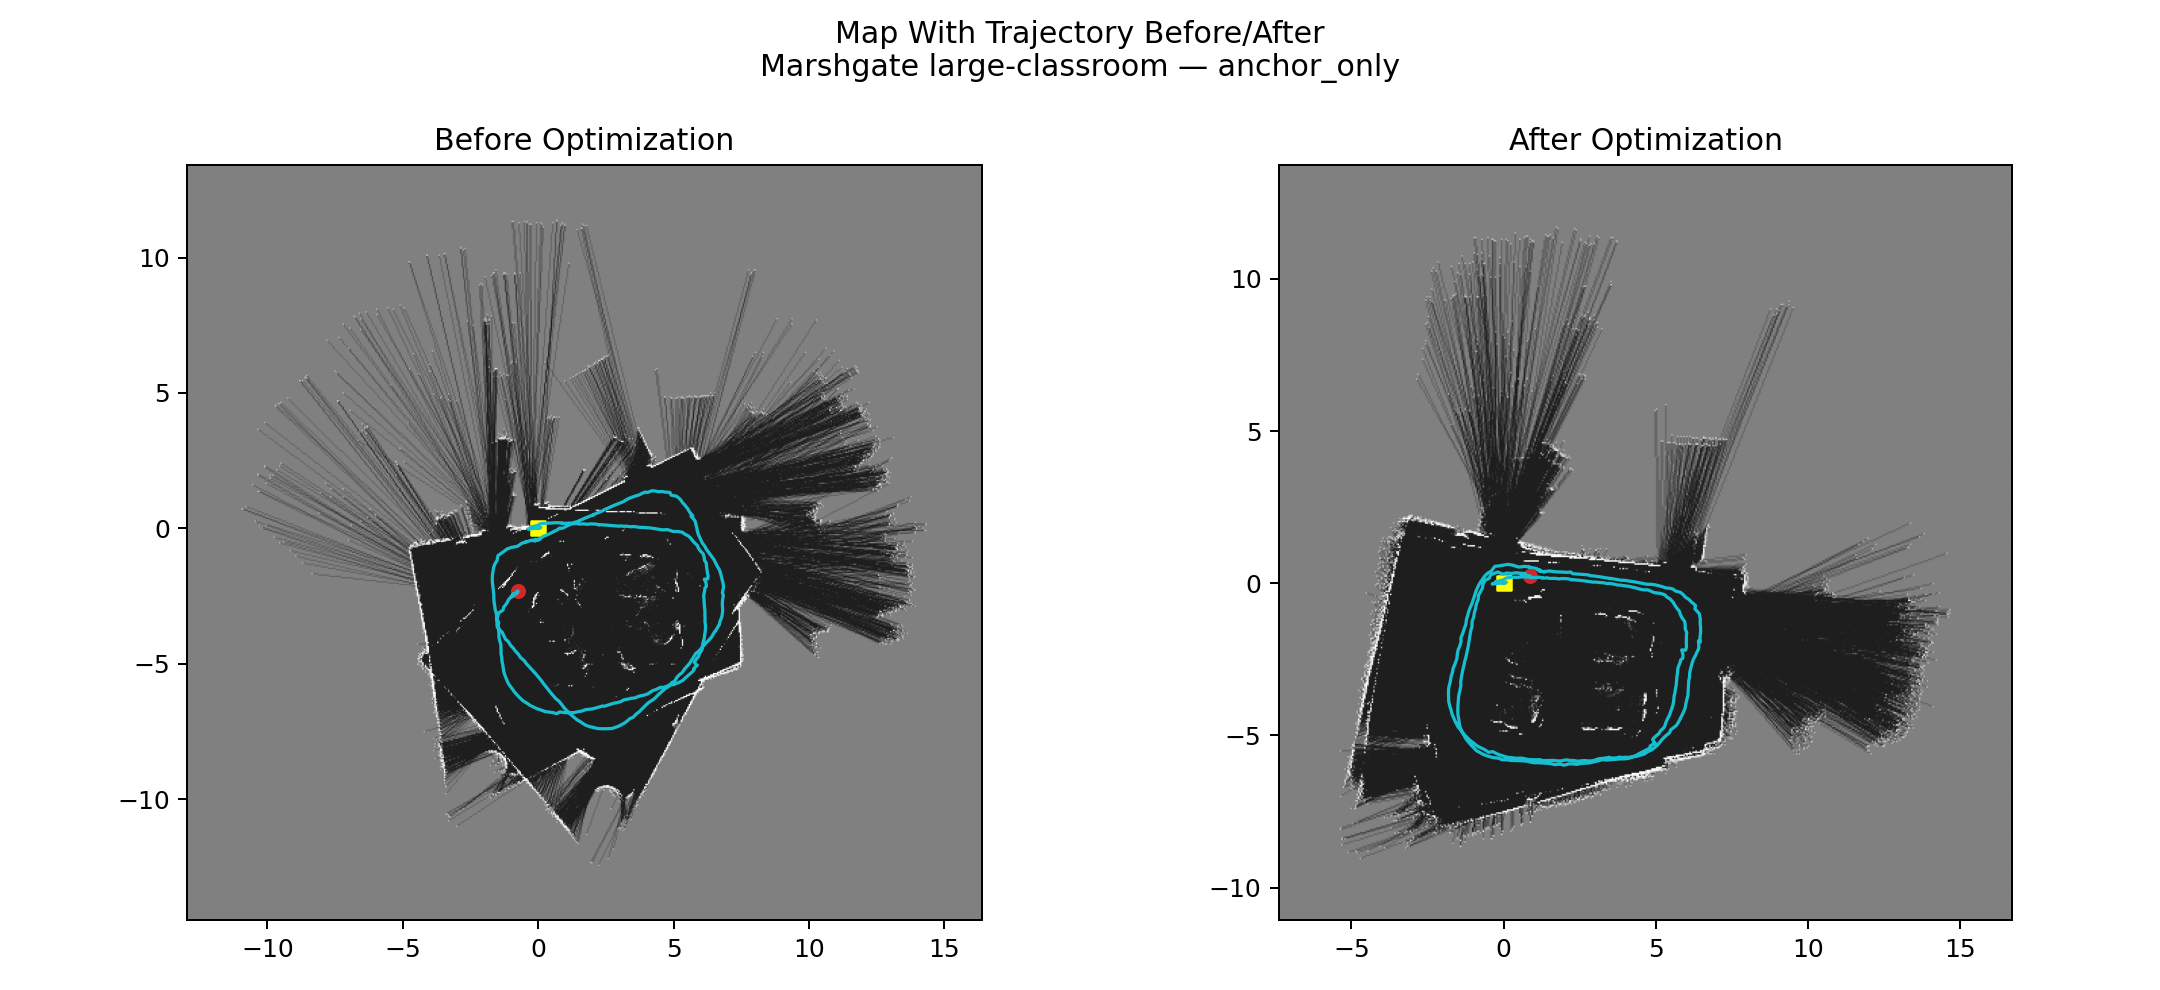
\includegraphics[width=\columnwidth]{images/Q3/optim_indoor_large.png}
\caption{Large indoor area before and after optimisation. The final pose moves much closer to the start.}
\label{fig:q3_optim_large}
\end{figure}

\begin{figure}[!htbp]
\centering
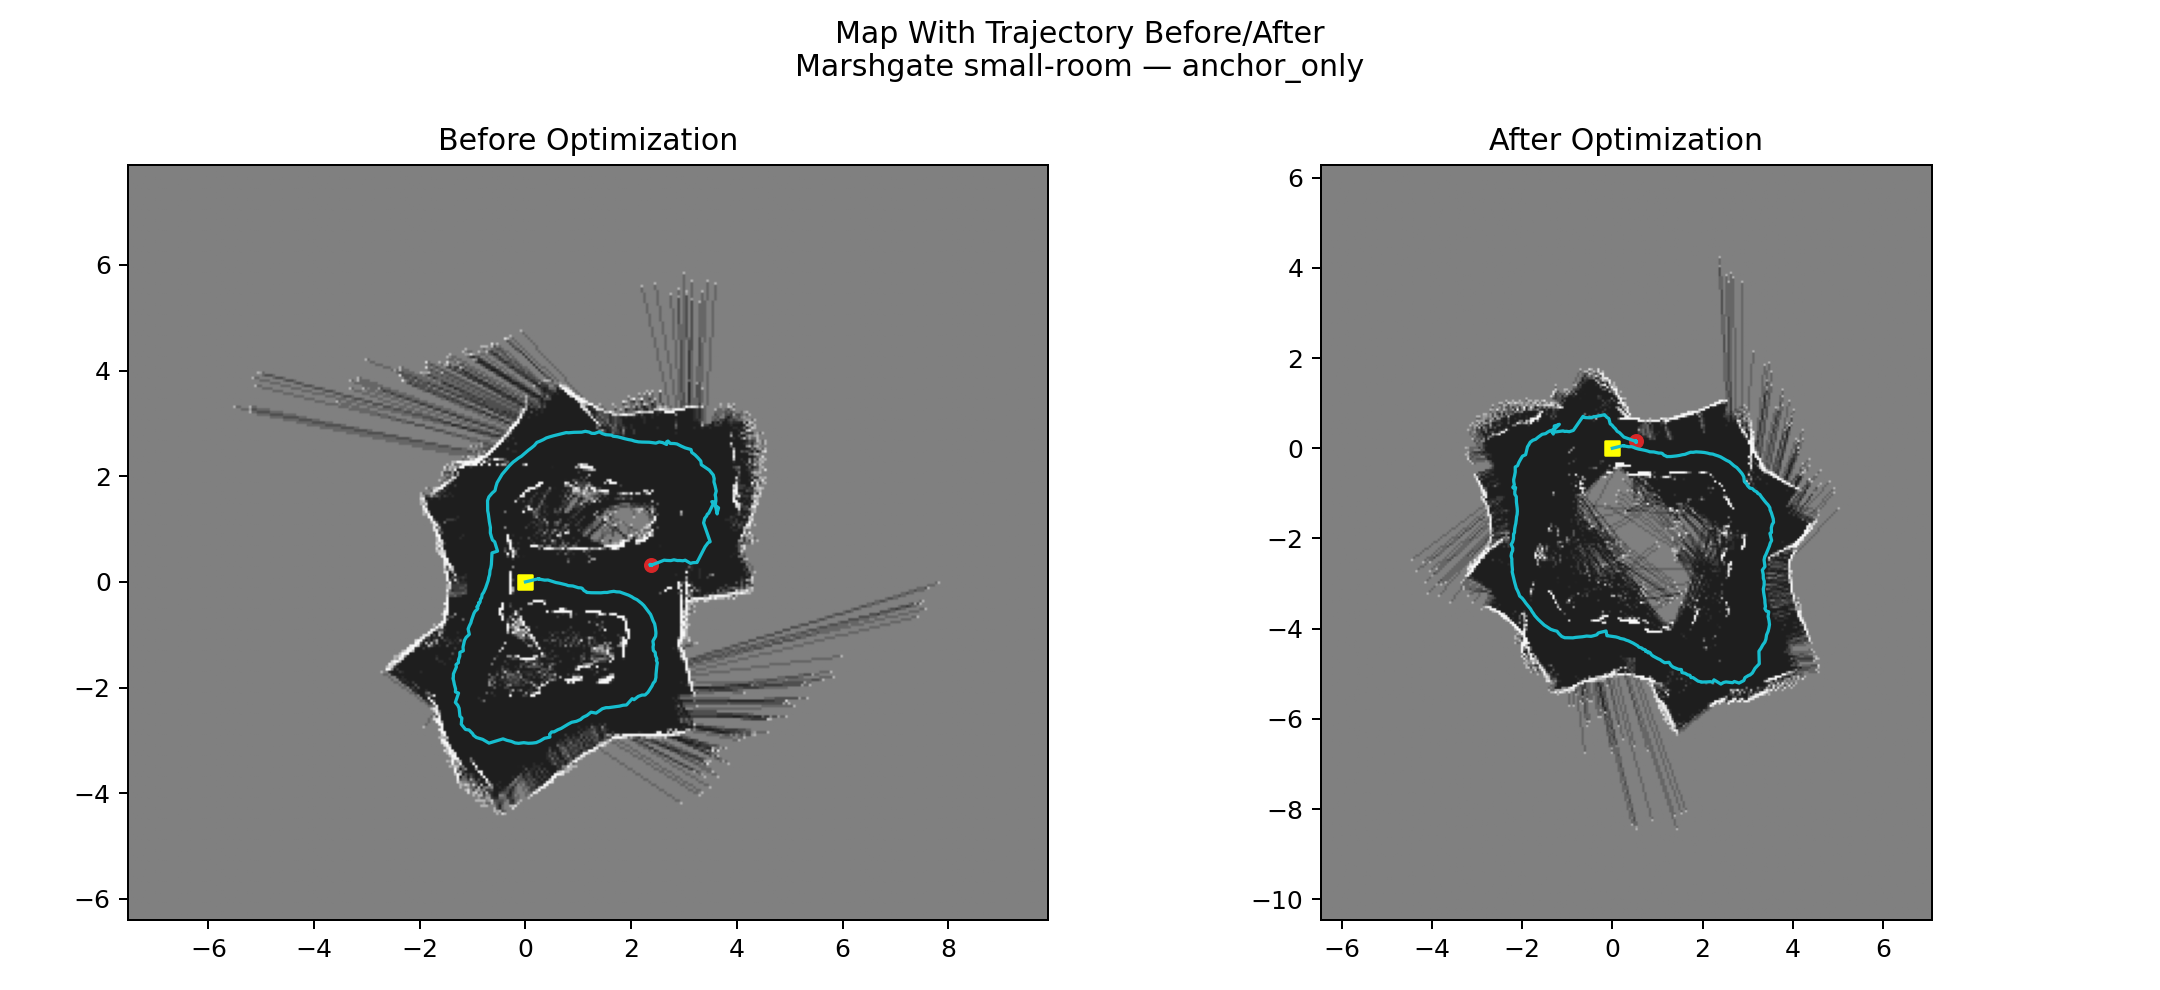
\includegraphics[width=\columnwidth]{images/Q3/optim_indoor_small.png}
\caption{Small indoor room before and after optimisation. The compact route closes much better after correction.}
\label{fig:q3_optim_small}
\end{figure}

For the outdoor route, one anchor loop alone also reduced the final error, but it bent the trajectory too much. The final result therefore uses one anchor loop and one supporting loop. Fig.~\ref{fig:q3_optim_outdoor} shows that the corrected trajectory returns much closer to the start, reducing the error from 2.820 m to 0.817 m. The outdoor map still has some duplicated and smeared structure, but it is clearly more consistent than the odometry-only map.

\begin{figure}[!htbp]
\centering
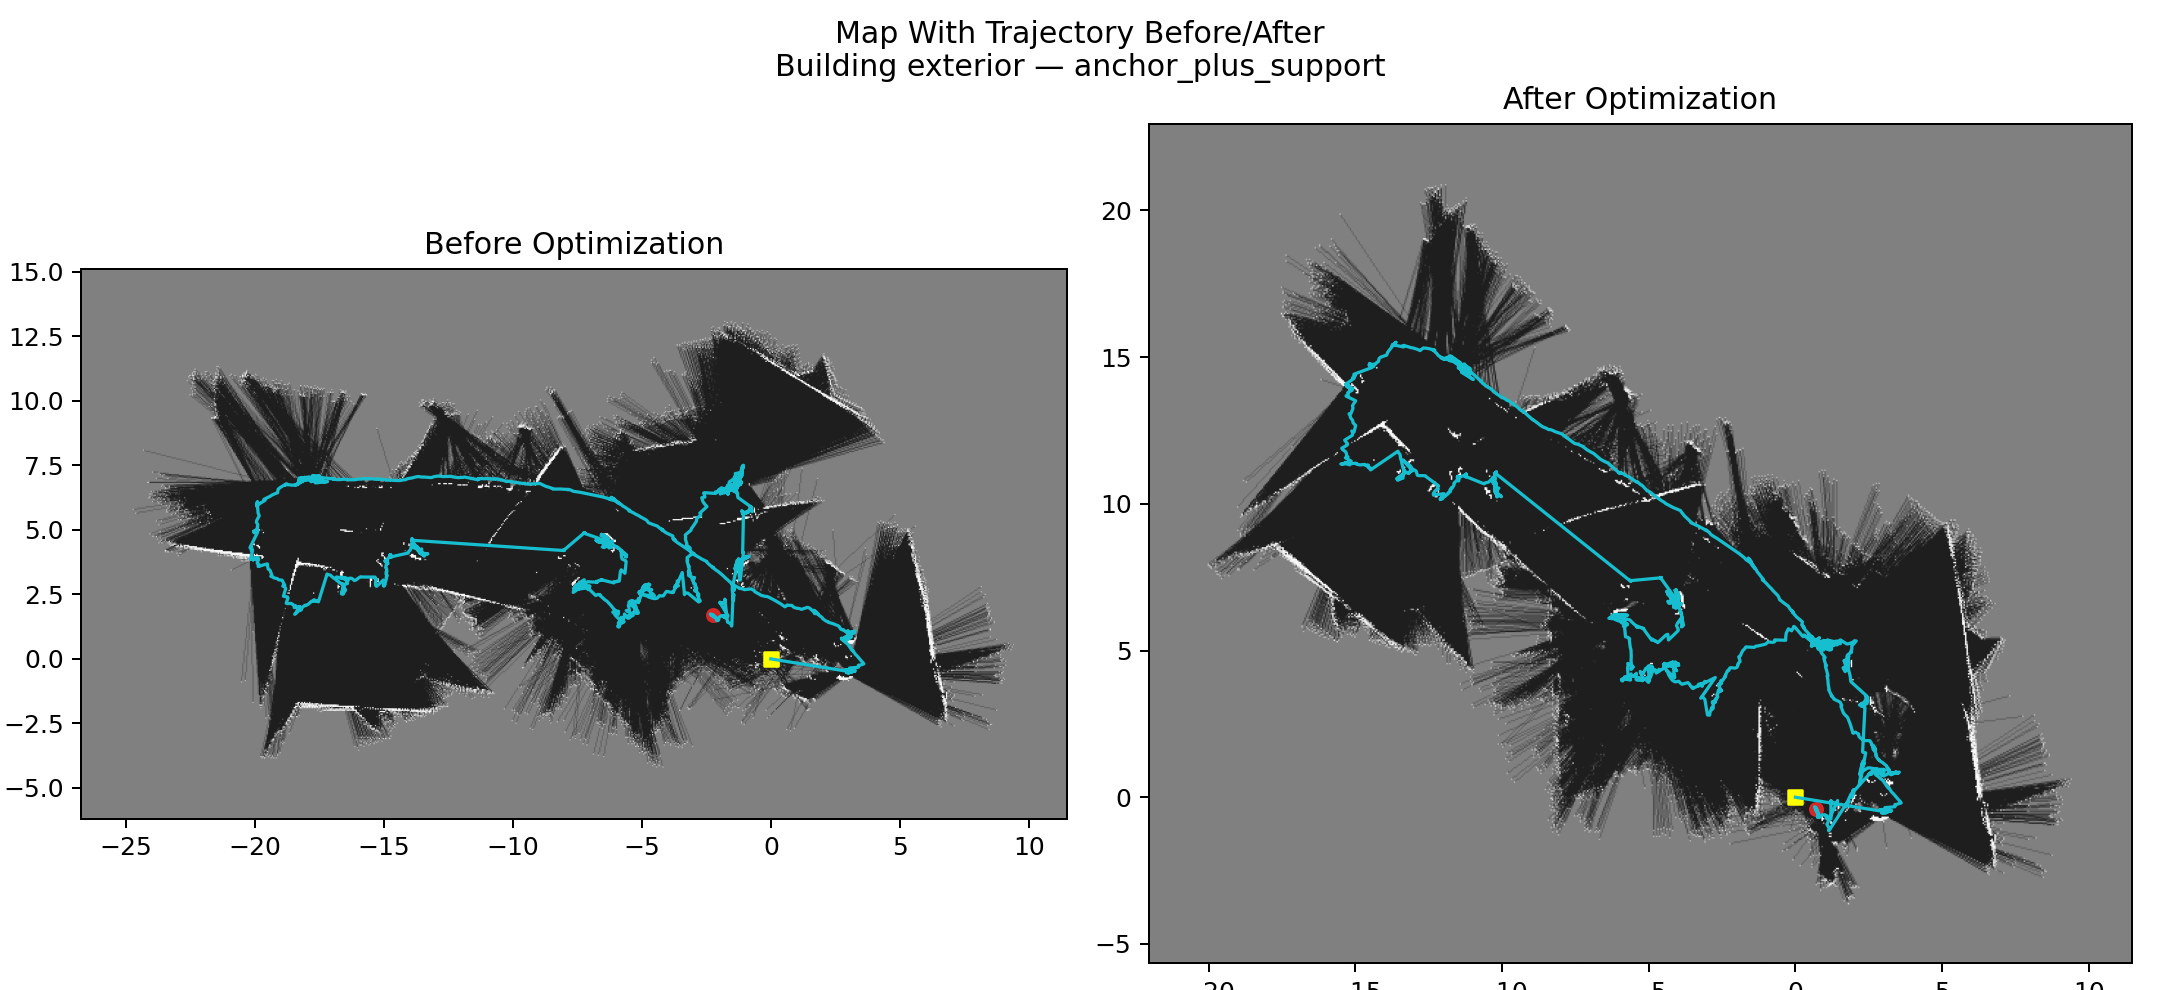
\includegraphics[width=\columnwidth]{images/Q3/optim_outdoor.png}
\caption{Outdoor route before and after optimisation. Two loop edges close the route while keeping the long trajectory smoother.}
\label{fig:q3_optim_outdoor}
\end{figure}

\subsection{Video Evidence and Discussion}

The submitted video shows the best LiDAR mapping run for each sequence. It includes the live map and the estimated path, so the second-loop consistency can be checked visually. The videos support the same conclusion as the numbers: laser odometry can build useful maps, but loop closure is needed to make the final loop consistent.

\FloatBarrier

% ============================================================
\section{Conclusion}
\label{sec:conclusion}

This report presents the group coursework results for visual and LiDAR SLAM. For the self-collected visual sequences, the outdoor route agreed better between COLMAP and ORB-SLAM2 because it had sharper images and clearer visual structure. The indoor route was harder because of low texture and repeated planar regions. For LiDAR SLAM, the parameter studies showed that good settings depend on the environment: longer range helped indoors but hurt outdoors, fine voxel filtering was important, and reduced scan rate helped some recordings but was not a general rule. Loop closure and optimisation reduced final drift in all three LiDAR sequences, from 2.443 m to 0.898 m in the large indoor area, from 2.395 m to 0.546 m in the small indoor room, and from 2.820 m to 0.817 m outdoors.

% ============================================================
% Optional bibliography placeholder. Add references if required.
% \begin{thebibliography}{00}
% \bibitem{orbslam2} R. Mur-Artal and J. D. Tardos, ``ORB-SLAM2: An Open-Source SLAM System for Monocular, Stereo, and RGB-D Cameras,'' IEEE Transactions on Robotics, 2017.
% \bibitem{colmap} J. L. Schonberger and J.-M. Frahm, ``Structure-from-Motion Revisited,'' CVPR, 2016.
% \end{thebibliography}

\end{document}
